%*****************************************
\chapter{État de l'art}\label{ch:psycho_ea}
%*****************************************


Avant d'aller plus loin dans l'exposé de nos travaux, il nous semble indispensable de dresser ici un état des lieux des connaissances liées à la perception des sons. Nous procédons en cinq parties. 

Au cours de la première, nous proposons un tableau général des différents processus intervenant dans le traitement de l'information sonore, processus mis en œuvre dès lors que le signal atteint le tympan. 

Au cours de la seconde, nous interrogeons la manière dont nous nous représentons le monde sonore perçu. Nous démontrons comment cette représentation influe sur notre perception. 

Au cours de la troisième, nous nous intéressons aux processus dits d'Analyse de Scènes Acoustiques (ASA), processus par lesquels le système auditif ségrègue les informations contenues dans l'environnement sonore afin d'en dégager des objets cohérents. 

Au cours de la quatrième, nous introduisons la notion de paysage sonore, et examinons l'impact que cette notion a sur les recherches en matière de perception des environnements. Nos travaux s'inscrivant largement dans cette approche, nous dressons un état de l'art des connaissances en matière de perception des paysages sonores, et tentons de dégager les grands axes méthodologiques suivis par ces études.

Au cours de la cinquième et dernière partie de cet état des lieux, sont précisés les concepts d'événement et de texture sonore, notions clefs qui interviennent par la suite dans le modèle de scène sonore proposé.

\gl{TODO: moins de "nous"}

\section{Le traitement de l'information auditive}

\subsection{La chaîne de traitement}
\label{sec:chaineTaite}

Le son est une vibration émise par une source d'excitation, et transmise à l'air. Cette vibration se propage ensuite jusqu'à atteindre un récepteur, le tympan, qui va capter le différentiel de pression résultant de cette vibration. C'est le point de départ du processus de traitement de l'information auditive. 

Si on adopte une approche \emph{traitement de l'information}, on peut décomposer ce processus en plusieurs systèmes interconnectés. Ces systèmes forment une chaîne qui, au fur et à mesure des traitements, interprète le signal acoustique afin d'en extraire l'information sémantique. Plus on se place loin dans la chaîne de traitement, plus on a accès à une information abstraite, potentiellement utilisable par d'autres processus de haut niveau. La figure \ref{fig:traitementSonMcAdamsBigand} extraite de \citep{mcadams1994penser} nous donne un aperçu des principales fonctionnalités du système de traitement auditif.

\begin{figure}[t]
        \myfloatalign
        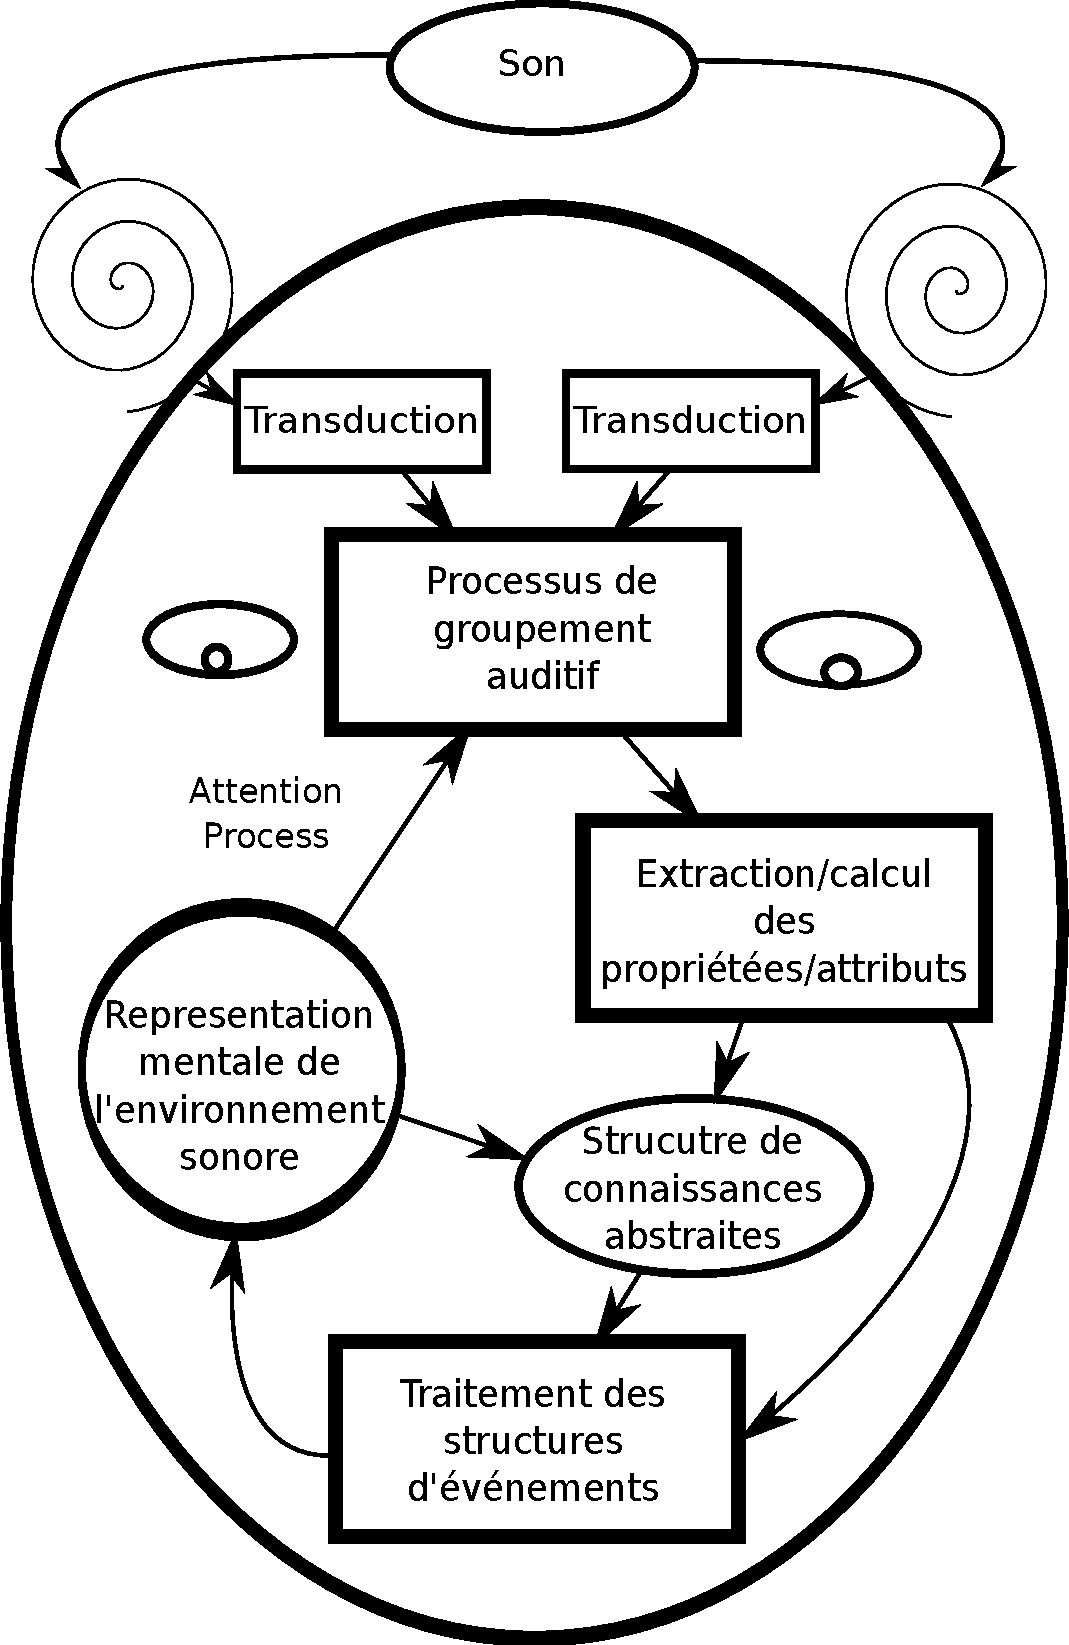
\includegraphics[width=.6\linewidth]{gfx/ch_3/traitementSonMcAdamsBigand}
        \caption[Principaux processus de traitement de l'information auditive et leurs interactions]{Principaux processus de traitement de l'information auditive et leurs interactions, d'après \citep{mcadams1994penser}}\label{fig:traitementSonMcAdamsBigand}
\end{figure}

\jls{perso ici je procèderais par énumération: La transduction..., Le groupement auditif..., L'extraction/calcul des propriétés... etc.}
Lors de l'étape de \emph{transduction}, les vibrations sonores parvenant au tympan, sont analysées puis traduites en impulsions nerveuses transmises au cerveau. Ces impulsions rendent compte des attributs spectraux et temporels de l'onde. L'extraction des composantes fréquentielles intervient dans la cochlée. C'est à l'intérieur de cette dernière que les différentes parties de la membrane basilaire vont être excitées, en fonction des fréquences composant le signal, suivant un axe tonotopique. Les vibrations, captées à chaque point d’excitation de la membrane basilaire, sont transmises au cerveau via les nerfs auditifs, chaque point codant une information correspondant à une bande fréquentielle limitée. 

Vient ensuite le \emph{processus de groupement auditif}. C'est une étape d'intégration temporelle au cours de laquelle l'information est analysée en images auditives cohérentes. Contrairement à ce que pensaient les Grecs anciens, nous ne possédons pas de "canaux" séparés pour chaque objet sonore présent dans l'environnement \citep{yost1994fundamentals}. C'est notre cerveau qui se charge de fusionner et de discrétiser les éléments sonores simultanés, afin de créer un flux auditif structuré. En d'autres termes, il détermine le nombre d'objets présents, identifie leur provenance, et en définit le sens. 

Afin d'illustrer notre propos, mettons nous dans la peau du mélomane écoutant \jlc{exit: "cette fois". Le "cette fois" suggère qu'il y a eu un  précédent. Quel est-il ?} un Choral de Bach. C'est le \emph{processus de groupement auditif} qui, sur la base des paramètres spectro-temporels du signal, nous permet de distinguer les voix de basse, ténor, alto et soprano. \jlc{Exit: Les travaux menés au titre de l'Analyse de Scènes Auditives (ASA), dont le sujet est abordé plus bas (\cf~Section~\ref{sec:ch3_ASA}), ont largement porté sur ces processus de groupement} \jls{perso je ne mettrais pas cette phrase. Aborder l'ASA ici est prématuré puisque tu traites le sujet plus loin. Et par ailleurs ça n'apporte pas grande précision, et ça casse le rythme de l'énumération. Et du coup, si on supprime, est-ce que tu peux commenter un tout petit peu "nous permet de distinguer BTAS" ?}.

Ces processus de groupement précèdent \jls{Le processus de groupement précède...} généralement la phase dite \emph{d'extraction/calcul des propriétés/attributs}. C'est lors de cette phase que sont extraites les qualités perceptives des objets groupés, ces qualités pouvant être vues comme des propriétés cognitives de haut niveau. Pour revenir au choral, c'est à partir d'une analyse des attributs perceptifs que nous sommes capables de percevoir les mélodies comme des objets unitaires, même si celles-ci sont développées entre les différentes voix.

Les phases de groupement et d'extraction concernent l'élaboration et l'analyse d'entités mentales. Une fois représentées dans le cerveau, ces entités sont interprétées pendant l'étape de \emph{structure des connaissances abstraites}. C'est lors de cette étape qu'elles sont identifiées, et qu'un sens interprétatif leur est donné. En pratique, il s'agit de déterminer si le Choral est plaisant ou non.

L'étape suivante, nommée \emph{Traitement des structures d'événements}, permet d'intégrer dans le processus cognitif différents contextes, comme par exemple le contexte fonctionnel (dans quel cadre ce son est-il entendu ?), ou encore le contexte sensoriel (l'information visuelle, ou la mémoire des événements sonores précédemment entendus). Pour revenir à notre mélomane, c'est cette étape qui lui permet d'envisager un morceau dans son ensemble, et, dans le cas d'une fugue, d'entendre que la strette finale est un résumé condensé des sujets précédemment exposés.

La dernière étape du processus de traitement est l'élaboration d'une représentation mentale de l'environnement perçu. C'est au cours de cette étape que nous organisons et conservons les différentes informations extraites. \jlc{La nature et la formation des représentations mentales sont abordées à la section~\ref{sec:ch3_representationMentale}} \jls{Comme plus haut, ça casse le rythme de ta présentation. Nous évoquerons la représentation mentale quand il en sera temps}.

\subsection{Processus \emph{Bottom-up} et processus \emph{Top-down}}
\label{sec:ch3_butd}

L'interaction entre l'homme et son environnement est fonction, d'une part, de l'information sensorielle captée par un individu, d'autre part, de la rétroaction exercée par lui sur ces données. 

\gl{\jlc{exit: Typiquement}, si nous reprenons la figure~\ref{sec:ch3_representationMentale}, les étapes de \emph{transduction} et de \emph{groupement auditif}, dépendent, entre autre, de la nature du signal perçu. \jlc{exit: À ce titre}, \jlv{ils mobilisent} \jlc{qui "mobilise" ? les étapes transduction et groupement auditif ? si oui alors "elles mobilisent"} des mécanismes innés, qui opèrent sur l'information sensorielle à partir de la présence de régularités physiques. Ces régularités sont universelles. Elles apparaissent quelle que soit la nature de l'environnement, et sont expérimentées par l'ensemble des individus. Par exemple, si la fréquence fondamentale d'un son harmonique change au cours du temps, toutes ses harmoniques changeront également afin de maintenir la structure harmonique du son [p. 38]\citep{bregman1994auditory} (\cf~Section~\ref{sec:ch3_regularitesEtProcessusPrimitifs}).}

\gl{La rétroaction, quant à elle, dépend de la mémoire de l'individu, \ie~sa représentation mentale interne des réalités externes du monde (\cf~Section~\ref{sec:ch3_representationMentale} et Figure~\ref{sec:ch3_representationMentale}). Cette mémoire est à la fois : }

\begin{itemize}
\item individuelle : déterminée par son expérience sensible, \ie~la mémoire des interactions sensorielles passées;
\item collective : déterminée par des connaissances transmises, connaissances qui dépendent de sa sphère d'appartenance socio-culturelle, ainsi que de sa langue maternelle.
\end{itemize}

\gl{C'est par l'interaction \jlc{tu as voulu dire: "C'est par la rétroaction" ?} que se manifeste l'expérience de l'individu, autrement dit, qu'il optimise l'analyse des stimuli, et intègre les effets de contexte dus à l'environnement. \jlv{Cette rétroaction est également l'expression de son individualité, individualité qui explique que deux personnes, ayant des capacités sensorielles semblables, peuvent percevoir différemment un même environnement} \jls{Cette rétroaction est également l'expression de son individualité. C'est l'individualité qui explique que deux personnes ayant des capacités sensorielles semblables peuvent percevoir différemment un même environnement}.} 

Le système auditif mobilise ainsi deux formes de traitements (\cf~Figure~\ref{fig:processusPercepAndCo}) :

\begin{itemize}
\item les traitements dits ascendants (\emph{bottom-up}), \gl{processus innés} et dirigés par les données;
\item les traitements dits descendants (\emph{top-down}) dirigés par les concepts ou les représentations.
\end{itemize}

Un exemple concret, emprunté au domaine de la vision, est celui du phénomène dit de bi-stabilité, \ie~la faculté, chez un sujet, de tirer d'un même stimulus deux analyses différentes, mais jamais simultanément \citep{schwartz2012multistability} (\cf~Figure~\ref{fig:bistabilite}). \\

\begin{figure}[t]
        \myfloatalign
        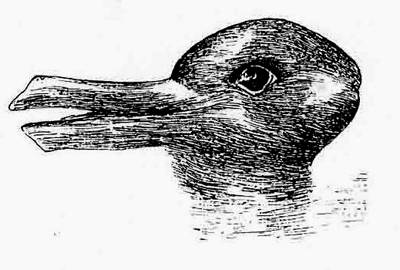
\includegraphics[width=.6\linewidth]{gfx/ch_3/canard_lapin}
        \caption[Le phénomène de bistabilité: l'illusion du canard-lapin]{Le phénomène de bistabilité: l'illusion du canard-lapin. Première publication dans \emph{Fliegende Blätter}, 23 octobre 1892, p. 147}\label{fig:bistabilite}
\end{figure}

Un autre exemple, emprunté cette fois au domaine de l'audition, nous semble illustrer encore le caractère dual de l'analyse de l'information sensorielle. Il est donné par McAdams et Bigand \citep[p. 2]{mcadams1994penser}:

\begin{quote}
``\,...Imaginez vous un instant en pleine forêt amazonienne : vous entendriez exactement les mêmes bruits que le guide qui vous accompagne, mais, étant donné votre manque de connaissance du milieu, vous seriez incapable d'extraire du fond sonore les sons correspondant aux cris de l'iguane, aux singes macaques, aux chants des ouistitis ou aux bruissements des arbres tropicaux. De ce fait vous seriez dans l'incapacité d'attribuer une signification à l'ensemble de la structure sonore, ce qui pourrait être important pour votre survie dans l'environnement.\,''
\end{quote}

Étudier le système auditif demande de prendre en compte aussi bien l'information externe (processus ascendant) que l'information interne (processus descendant). \gl{Réduire la perception à une simple association de sensations établies à partir du signal capté, ne permet pas de rendre compte de l'éventail des processus cognitifs entrant dans le décodage de l'environnement. Cette distinction entre perception et cognition est approfondie à la section suivante (\cf~Section~\ref{sec:ch3_perceptionCognition})}. \\

\gl{TODO: plus de liens avec la figure~\ref{sec:ch3_representationMentale} ?}

\subsection{Perception et cognition}
\label{sec:ch3_perceptionCognition}

Perception. Le mot désigne l'ensemble des processus de traitement de l'information sensorielle. La perception du monde sonore qui nous entoure est un phénomène complexe, aujourd'hui encore mal connu. 

Cette perception est à l'origine de l'interaction que nous créons avec notre environnement. Elle détermine notre capacité d'adaptation à ce dernier. Cette relation au monde \emph{réel} ne se rompt jamais. Nous percevons des sons en permanence, et ce, même si aucune source sonore n'est présente. 

Ainsi tel mélomane dont la tête résonne encore de l'air, bien après que les instruments se soient tus. Ainsi tel usager des transports dont l'oreille anticipe (pour s'en protéger...) les crissements du métro alors que la rame n'est pas encore à quai.

Cognition. Selon U. Neisser\footnote{Ulric Neisser est considéré comme un des pères du cognitivisme notamment grâce à son livre \citep{neisser1967cognitive}. Il a par la suite critiqué la direction prise par le mouvement, dénonçant une "approche laboratoire" trop éloignée de la réalité terrain.} dans \citep[p. ??]{neisser1976cognition}:

\begin{quote}
``\,Cognition is the activity of knowing : the acquisition, organisation and use of knowledge.\,''
\end{quote}

Le mot désigne l'ensemble des processus d'acquisition et de développement d'une connaissance du monde. 

Selon la théorie classique, perception et cognition dépendent de deux groupes de systèmes fonctionnels du cerveau distincts. La perception mobilise les systèmes de traitement dits modaux, c'est à dire supportés par les organes sensoriels (oreilles, yeux etc $\ldots$), tandis que la cognition s'appuie sur des représentations mentales des réalités externes, par essence amodales.
 
Cette dichotomie entre perception et cognition est aujourd'hui remise en question. Dans une approche ``\,incarnée\,'' de la cognition (\emph{Grounded Cognition}), Barsalou nie le caractère amodal des représentations mentales prônant que ces dernières dépendent également des modalités sensorielles \citep{barsalou2010grounded}. Il tente ainsi de réunir les processus perceptifs et cognitifs \citep{goldstone1998reuniting, barsalou1999perceptions}.

Les deux approches sont illustrées sur la Figure~\ref{fig:processusPercepAndCo}.

\begin{figure}[t]
        \myfloatalign
        \includegraphics[width=.8\linewidth]{gfx/ch_3/Representation}
        \caption{Processus cognitifs et perceptifs}\label{fig:processusPercepAndCo}
\end{figure}

\subsubsection{Psychologie cognitive et psychoacoustique}

La psychologie cognitive est un domaine de recherche dédié aux phénomènes se rapportant à la connaissance. Elle est née dans les années 50, en réaction au \emph{Béhaviorisme}, théorie fondée sur ``\,l'étude des comportements objectivement observables de l'être humain\,'', et négligeant, de fait, le rôle de la conscience. La psychologie cognitive s'interroge sur des modèles théoriques complexes rendant compte de tous les faits et de toutes les lois connus. Les chercheurs y explorent tout à la fois, la mémoire, le langage, l'intelligence, la perception.
 
L'approche cognitiviste, dans le domaine de la perception auditive, se distingue de celle plus traditionnelle de la psychoacoustique \footnote{La psychoacoustique est une branche de la psychophysique qui applique au domaine de l'acoustique les concepts et les méthodes de la psychophysique}. Tandis que la psychoacoustique émet l'hypothèse d'une relation directe entre le stimulus et la réponse du sujet, la psychologie cognitive soutient que la réponse, elle, est entièrement corrélée au contexte, à l'expérience, et aux interactions multi-sensorielles \citep{maffiolo_marieParis_1997}.

La réponse tient compte non seulement des traitements perceptifs mais aussi des représentations issues et de la mémoire individuelle (\ie~construites en particulier à partir de la relation sensible au monde), et de la mémoire collective, à travers le développement des connaissances partagées \citep[p. ??]{maffiolo_caracterisation_1999}.

La psychologie cognitive s'intéresse prioritairement à l'aspect cognitif de la perception en considérant l'individu comme un tout. Elle prend en compte la culture, l'expérience, l'activité de l'individu et ne focalise pas seulement sur la réaction des organes sensoriels comme l'oreille. Elle questionne les aspects qualitatifs plus que quantitatifs de notre compréhension du monde sonore \citep[p. ??]{maffiolo_caracterisation_1999}.

Elle envisage l'ensemble des étapes du traitement auditif de manière globale et permet ainsi de faire le lien entre une information sensorielle et une information abstraite \citep{mcadams1994penser}.

En psychologie cognitive, on distingue les approches cognitivistes, qui s'intéressent plus particulièrement aux processus montants (\emph{botttom-up}, \cf~Section~\ref{sec:ch3_butd}), relatifs au traitement de l'information perçue, et les approches cognitives, qui interrogent, avant tout, les processus descendants (\emph{top-down}, \cf~Section~\ref{sec:ch3_butd}) liés à la mémoire du sujet ainsi qu'au contexte \citep[p. ??]{guastavino_etude_2003}.

\subsubsection{Paradigme de la psychologie cognitive}
\label{sec:ch3_psychoCog}

\jlv{Nous l'avons vu} \jls{Nous le voyons}, la psychologie cognitive ne conçoit pas le sujet comme une ``\,boîte noire\,'', mais reconnaît en lui un système de traitement de l'information. Elle admet que l'individu adopte une stratégie afin d'optimiser le traitement des stimuli. Cette stratégie est déterminée par la nature du stimulus, mais aussi par son contexte, et par les connaissances a priori du sujet.

Maffiolo \citep[p. ??]{maffiolo_caracterisation_1999} propose une présentation des présupposés sur lesquels repose la psychologie cognitive (\cf~Figure~\ref{fig:paradigmeCognitivisme}). Ces présupposés sont résumés ci-après:

\begin{itemize}
\item le monde est discrétisé en dimensions ou propriétés issues de la physique, et considérées comme vraies;
\item ces dimensions ou propriétés peuvent être mesurées objectivement par des instruments. Elles rendent compte ainsi de la réalité;
\item le sujet intègre de manière séquentielle ces dimensions ou propriétés en fonction du contexte;
\item l'évaluation subjective du sujet est interprétée comme un décalage par rapport à la mesure objective considérée comme vraie.
\end{itemize}

\gl{\jlv{Ce paradigme} \jlc{On est dans l'énumération des présupposés de Maffiolo. De quel paradigme parles-tu ?} repose sur la dualité communément acceptée en psychologie entre subjectivité et objectivité, autrement dit, la différenciation opérée entre, d'un côté, le monde ``\,réel\,'' (et \emph{a fortiori} les objets qui le composent), et, de l'autre côté, le sujet.}

Au regard de ce paradigme, Maffiolo met en évidence quatre points discutables :

\begin{enumerate}
\item la pertinence des dimensions et propriétés physiques utilisées pour le découpage du monde; 
\item un traitement par les sujets tenant spécifiquement compte de ces dimensions;
\item une séparation nette entre stimulus et contexte;
\item le caractère subjectif du jugement humain en comparaison à l'objectivité d'un appareil de mesure.
\end{enumerate}

\gl{Les points 1 et 2 se rejoignent. Les dimensions physiques utilisées pour décrire le monde sont établies par les sciences naturelles, \emph{via} des procédés qui ne prennent pas en compte la perception du sujet. Dans le cas de l'analyse sensorielle, questionner la pertinence de ces dimensions,  \ie~leur capacité à diriger notre relation sensible au monde, est \jlc{exit: donc} naturelle. Il est \jlc{exit: notoirement} connu aujourd'hui que ces dimensions ne peuvent expliquer seules les processus perceptifs mis en œuvre, notamment pour ce qui est de l'audition et de l'olfaction \citep{dubois2000categories}. On peut citer ici la capacité limitée des descripteurs psychoacoustiques comme la \emph{loudness} (\cf~Section~\ref{sec:ch3_appCatDim}) a caractériser l'intensité perçue, et encore plus, la gêne occasionnée par cette intensité, pour des stimuli réels enregistrés (\cf~Section~\ref{sec:ch3_urbanNoiseSoundscape}).} \\

\gl{TODO: a) perception dépend d'autres caractéristiques, b) construction de la loudness à partir de sons purs.} \\

\gl{Concernant le point 3, bien que le paradigme suppose l'influence d'un contexte, ce dernier est considéré comme une entité séparée du stimulus, un élément modificateur qui agirait sur la perception de ce dernier. Ce fait implique qu'il existe une représentation mentale de l'objet perçu (\ie~le stimulus), déconnectée de tout contexte d'exposition. Un objet n'étant jamais perçu de manière isolé, ce point peut être à juste titre considéré comme une hypothèse très restrictive.} 

\gl{Enfin, le fait de considérer les réponses ``\,subjectives\,'' du sujet comme une déviation par rapport à une réalité physique externe implique que le monde  est indépendant des représentations mentales que nous nous en faisons, et qu'il est possible d'en ``\,trier\,'' l'information sans tenir compte de la manière dont nous l'interprétons \citep{dubois2000categories}. \jlc{exit: Par là même}, cela suppose que l'existence des objets qui composent le monde est avérée, et indépendante de notre perception. Or, comme nous le verrons \jlc{exit: dans tout au long de ce document}, la perception d'un objet varie \jlc{exit: grandement} d'un sujet à l'autre, que l'on considère son identification (Quel est l'objet perçu ?), sa description (Comment et à partir de quels descripteurs l'objet est-il perçu ?) ou son interprétation (Quel est l'effet de l'objet sur le sujet ?). Questionner ce dernier point revient ainsi à se poser la question suivante:}
\jlc{ici, l'emploi de l'itemize n'est pas indiqué}. \jls{Questionner ce dernier point revient à interroger: "Est-ce que l'objet existe parce que je le perçois, ou est-ce que je le perçois parce qu'il existe ?}
\begin{itemize}
\item Est-ce que l'objet existe parce que je le perçois, ou est-ce parce que je le perçois, que l'objet existe ?
\end{itemize}

\gl{Toutes ces questions/remarques restent ouvertes. Loin de dénigrer l'approche de la psychologie cognitive, elles doivent être vues comme des aides, et prises en compte dans l'interprétation des résultats d'expériences reposant sur ce paradigme.}\\

\gl{TODO: faire le lien ici avec les descripteurs subjectifs utilisé pour caractériser un environnement sonore}

\begin{figure}[t]
        \myfloatalign
        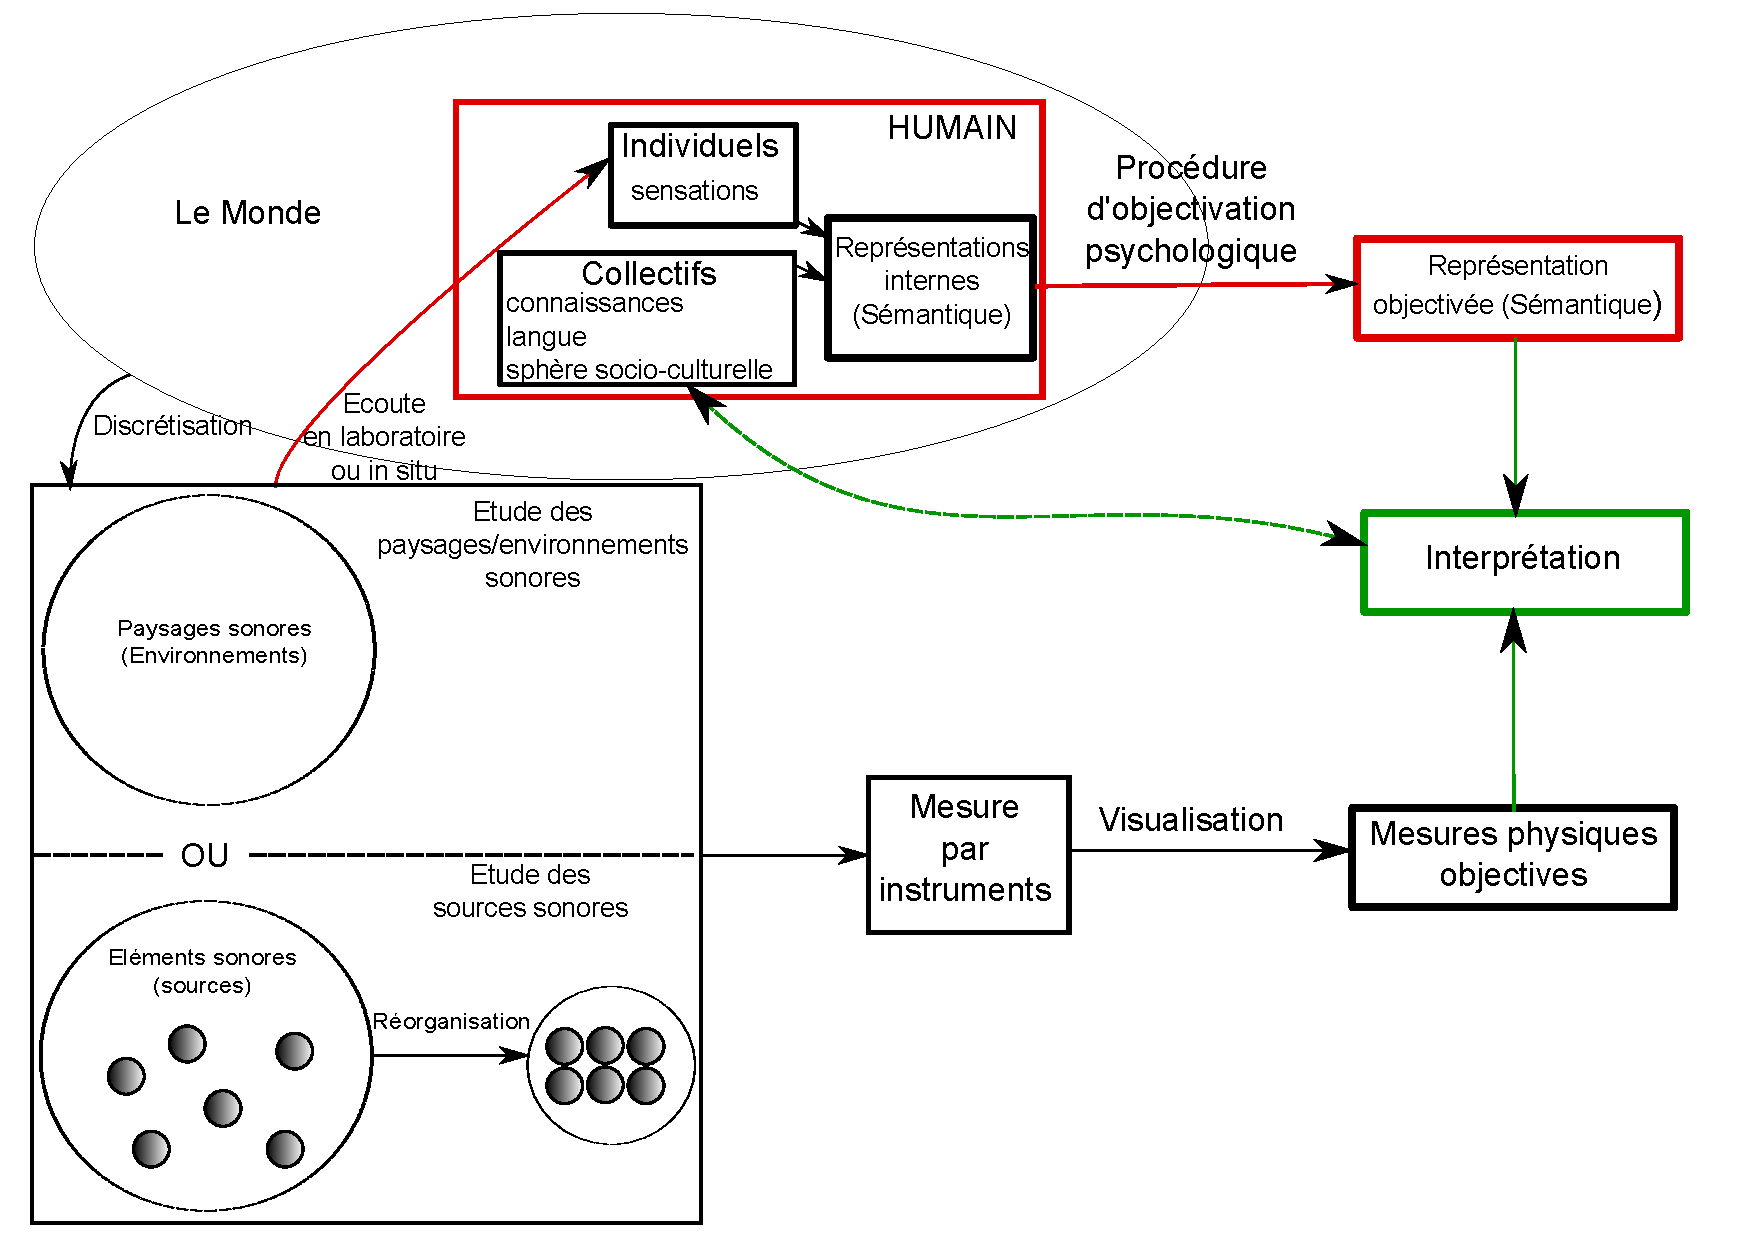
\includegraphics[width=\linewidth]{gfx/ch_3/Shema_maffiolo}
        \caption[Paradigme de la psychologie cognitive]{Paradigme de la psychologie cognitive, d'après \citep{maffiolo_caracterisation_1999} \gl{à quoi réfèrent les adjectifs individuels et collectifs ?}}\label{fig:paradigmePsychoCo}
\end{figure}

\subsection{L'approche écologique}
\label{sec:ch3_ecologique}

L'approche écologique a d'abord été introduite dans le domaine de la vision par Gibson \citep{gibson1966senses}, qui se demande entre autre si les ``\,lois structurant les objets sont porteuses d'informations, ou si cette information est tirée de comparaisons \,'' \citep{gibson1978ecological}.

Cette approche reconnaît que la réponse au stimulus dépend à la fois de l'information perçue, et de la connaissance du monde, autrement dit, l'environnement quotidien, et le contexte habituel d'écoute du stimulus.

\subsubsection{\emph{Soundwalk}}

Appliquée à la perception sonore, l'approche écologique requiert de prendre en compte l'environnement et du sujet, et du stimulus auquel il est exposé. La démarche s'oppose aux méthodes expérimentales traditionnelles, celle de la psychophysique en particulier, sur l'aspect décontextualisant de l'écoute en laboratoire, qui affecte la perception du sujet contraint à un effort d'abstraction supplémentaire pour obtenir l'illusion de la réalité.

Nombre d'études désormais sont réalisées dans un cadre \emph{in situ}. On parle d'ailleurs de \emph{soundwalk}  \footnote{\emph{Soundwalk} est un terme anglais introduit par R. Murray Schafer \citep{schafer1969new} signifiant littéralement ``\,marche sonore\,''. Ce terme étant couramment utilisé en français, il ne sera pas traduit dans ce document.} pour désigner les expériences où le sujet est immergé dans l'environnement qu'il doit évaluer \citep{adams2008soundwalking,jeon2013soundwalk}.


La méthode des \emph{soundwalk} permet entre autre:

\begin{itemize}
\item  de contextualiser le sujet, à savoir, l'évaluer dans un environnement qu'il connaît (lieu de vie, de travail);
\item d'évaluer l'environnement sonore, tout en maintenant actif les autres sens (vue, olfaction);
\item d'éluder le problème de la reproduction des environnements sonores en laboratoire.
\end{itemize}

Malgré tout, les études \emph{in situ}, bien que valides écologiquement, présentent elles aussi des inconvénients. Dans l'hypothèse où tous les sujets ne passent pas l'expérience en même temps, il est impossible de garantir à chacun les mêmes stimuli et/ou le même environnement. Se pose le problème de la reproductibilité des expériences. Inversement, dans l'hypothèse où tous les sujets passent l'expérience en même temps, il peut se poser des problèmes d'organisation, de nature à compromettre une égale réceptivité, disponibilité chez tous les sujets.

\subsubsection{Reproduction écologique des environnements sonores en laboratoire}

Le problème de la reproduction écologique des environnements sonores en laboratoire a été particulièrement étudié par Guastavino. \citep{guastavino2003approche,guastavino2004perceptual,guastavino2005ecological}. En comparant les descriptions verbales produites à la suite d'écoutes \emph{in situ} , et d'écoutes en laboratoire, via des systèmes de reproduction stéréophoniques et multi-phoniques, \citep{guastavino2005ecological} montre que les événements sonores peuplant les scènes sont décrits de la même manière, quel que soit le contexte d'écoute.

Cependant des différences apparaissent au niveau de la description des fonds sonores (\emph{backgrounds}), entre les écoutes stéréophoniques, et les écoutes multi-phoniques et \emph{in situ}, suggérant de fait que le système de reproduction influe sur les processus cognitifs mis en œuvre. Des conclusions similaires sont faites dans \citep{guastavino2004perceptual} s'agissant cette fois de systèmes de reproduction mono, stéréo, et multi-phoniques. \\

\gl{TODO: sélection des stimuli} \\



\section{Représentation mentale de l'environnement sonore}
\label{sec:ch3_representationMentale}
 
\gl{TODO: être moins prétentieux, ajouter "il semble, il est utile, il est communément admis"}
 
Le cerveau entretient un dialogue constant avec l'environnement sonore. Ce dialogue s'effectue par le biais des représentations mentales. Une définition des représentations mentales est donnée par \citep{houde1998vocabulaire}:

\begin{quote}
``\,La représentation mentale peut être vue comme une entité interne, le correspondant cognitif individuel des réalités externes expérimentées par un sujet.\,''
\end{quote}

Ces représentations font office de sauvegardes de l'information. Conservées en mémoire sous une forme abstraite \citep[p. 357]{mcadams1994penser}, elles rendent compte à la fois de notre compréhension du monde, et de la manière dont nous l'abordons. Ces connaissances subjectives, non directement observables, restent néanmoins accessibles au chercheur par le biais d'expériences d'objectivation (voir section~\ref{sec:ch3_appCategorielle})
 
Ces représentations forment une image mentale discrète d'un \jls{du} monde réel continu \citep{houde1998vocabulaire}. C'est par le passage du continu au discret que nous sommes à même d'organiser nos connaissances, afin de les réutiliser de manière efficace. Les objets discrets, issus de cette organisation, sont appelés des catégories. L'action consistant à juger si un événement perçu appartient à une catégorie est appelée la catégorisation.

\subsection{La notion de catégorie}

\subsubsection{Définition}
\label{sec:ch3_categorieDef}

Une des vérités de tout être humain est de segmenter son environnement, \ie~de se bâtir un système de classification permettant de regrouper des objets n'étant pas identiques \citep[p. 1]{rosch1978cognition}. On appelle catégorisation, l'action consistant à regrouper des objets du monde physique considérés comme équivalents, et catégorie, l'entité mentale contenant le groupe d'objets ainsi rassemblés. 
 
D'un point de vue écologique, la catégorisation est un processus essentiel. Nous sommes constamment en train de catégoriser l'environnement, et devons être à même, à tout moment, de prendre une décision sur l'appartenance catégorielle d'un objet. Ce processus est adaptatif. La prise de décision est toujours fonction du sujet, d'une situation et d'un contexte. Ainsi, un même objet, perçu à deux moments distincts, pourra être affecté à des catégories différentes. 


\citep{anderson1991adaptive} propose trois exemples de manifestations quotidiennes des catégories:

\begin{itemize}

\item le langage: Le langage est le lieu, par excellence, des catégories. Catégoriser, c'est considérer un objet comme un élément distinct du monde. Cette distinction s'accompagne généralement (pas toujours) d'une désignation. C'est l'essence même des processus d'identification que de chercher à nommer les objets, une fois qu'ils ont été isolés. Il est raisonnable de penser que, de la même manière, une catégorie possède un label associé. On parlera alors de catégorie sémantique. Cette relation entre langage et catégorie nourrit le débat sur l'universalité présupposée de la catégorisation. L'opération permanente consistant à isoler un objet, et à lui attribuer un nom, est l'antinomie du ``\,geste adamique\,'', \ie~d'attribution libre du nom, hors toute influence et/ou contexte (d'Adam, le premier homme révélé et nommé dans la bible). La langue est un code partagé par une communauté. Dans une certaine mesure, sa définition, \ie~le sens donné aux mots, peut varier suivant les groupes de cette communauté. Ainsi, catégoriser ne dépend pas seulement d'une réalité physique du monde, mais également d'un contexte socioculturel. La catégorisation peut être vue comme une action intermédiaire entre, d'une part, l'organisation d'une connaissance individuelle résultant d'une expérience sensorielle personnelle, et, d'autre part, la constitution d'une représentation collective pouvant être partagée par le biais d'un langage commun \citep{dubois2006cognitive}.
\item le regroupement par similarité des caractéristiques: Nous sommes capables de regrouper des objets possédant des caractéristiques similaires, et ce, même si ces objets nous sont inconnus \citep{fried1984induction}.
\item le regroupement par similarité fonctionnelle: Nous sommes capables d'interpréter des objets possédant des fonctions similaires comme faisant partie d'un même groupe, et ce même si ces objets ont des caractéristiques distinctes. Pour exemple: deux hommes descendant d'un camion de pompier pour éteindre un feu de forêt seront catégorisés pompiers, ce indépendamment des tenues qu'ils portent. Quand nous parlons de la catégorisation comme du processus de discrétisation du monde réel, ce "monde réel" englobe et la réalité des faits physiques, et la réalité des faits sociologiques.
\end{itemize}

\subsubsection{La nature des catégories}

Toute opération permettant de ``\,voir un objet comme étant $\ldots$\,'' plutôt que de simplement ``\,voir un objet\,'' relève de la catégorisation. Tous les objets peuvent être catégorisés, quelle que soit leur nature \citep{goldstone2003concepts}. Reconnaître un animal comme étant un éléphant est un acte catégoriel. Identifier qu'un morceau de musique est le premier mouvement d'une sonate, et qu'il est issu de la période classique, relève également d'un processus de catégorisation. La catégorisation intervient donc sur des objets de différentes natures. On distingue généralement trois types de catégories:

\begin{itemize}
\item catégories naturelles: regroupent des objets existant à l'état naturel (animaux, fleurs, \etc);
\item catégories artificielles: regroupent des objets fabriqués par l'homme (voitures, outils);
\item catégories de concepts:  regroupent des objets abstraits qui ne sont pas ancrés dans une réalité physique (art, stratégie, sentiments).
\end{itemize}

Ces trois types de catégories groupent des objets sur la base de leurs similarités. Pour les catégories d'objets naturels et artificiels, ces similarités s'établissent majoritairement à partir de leurs caractéristiques physiques. Pour les catégories de concepts, ces similarités relèvent d'attributs cognitifs de plus haut niveau. De plus, qu'ils soient abstraits ou concrets, ces objets ont une existence avérée, \ie~indépendante du contexte.

Cependant, certaines situations particulières poussent à grouper des objets parfaitement dissimilaires, \eg~la liste de courses. Les catégories inhérentes à de tels groupements sont nommées \emph{ad hoc} \citep{barsalou1983ad}:

\begin{itemize}
 \item catégories \emph{ad hoc}: regroupent des objets afin de répondre à un besoin spécifique.
\end{itemize}

\subsection{Le processus de catégorisation}

\subsubsection{Catégorisation et prédiction}
\label{sec:ch3_categoPred}

La structure catégorielle forme la base des ressources cognitives sur lesquelles nous nous appuyons afin d'isoler des objets du monde. Ce processus procède de deux mécanismes:

\begin{itemize} 
\item mécanisme inductif: associer un objet à une catégorie sur la base des propriétés perçues de ce dernier;
\item mécanisme déductif: associer à un objet les propriétés de la catégorie à laquelle il appartient.
\end{itemize}

\jlc{exit: Le mécanisme déductif est d'une importance capitale}. \jlc{Tu finis par "Notre capacité d'adaptation est très liée...". C'est donc qu'il est important. Il n'y a pas besoin d'en rajouter} \jls{Le mécanisme déductif nous permet de généraliser nos connaissances...}. Il nous permet de généraliser nos connaissances, \ie~d'inférer les propriétés d'un objet sans pour autant les avoir perçues. Ces propriétés transmises peuvent être physiques ou conceptuelles. Exemple: il suffit de voir la croupe d'un cheval pour en "déduire" l'animal. Autre exemple: le bourdonnement d'un insecte peut laisser supposer la présence d'une guêpe, et susciter le sentiment du danger. On le voit, le mécanisme déductif nous permet d'aller au delà de l'information perçue, mais peut également mener à des erreurs d'interprétation. Notre capacité d’adaptation est très liée à ce mécanisme.

\subsubsection{Catégorie et langage}
\label{sec:ch3_catLang}

\gl{Comme nous l'avons vu (\cf~Section~\ref{sec:ch3_categorieDef}), catégorie et langage fonctionnent de concert. En attribuant le même nom a des objets distincts nous les regroupons \emph{de facto} dans la même catégorie.}

\gl{Les catégories n'étant pas accessibles directement par l'expérimentateur, l'analyse linguistique des descriptions verbales est un moyen d'objectiver les représentations mentales d'un individu (\cf~Section~\ref{sec:ch3_appCategorielle}).}

\jlv{Dans le domaine de l'audition, cette utilisation de l'analyse linguistique afin de comprendre les processus de catégorisation a particulièrement été étudiée par Dubois et ses collègues \citep{dubois2000categories,raimbault2005urban,dubois2006cognitive,guastavino2006ideal}. Leurs études montrent, entre autre, que, contrairement à la vision, il n'existe pas en audition (ainsi qu'en olfaction \citep{dubois2000categories}) de consensus entre les sujets sur le vocable à utiliser pour décrire les phénomènes sonores. En conséquence, l'analyse est pratiquée sur des descriptions verbales ayant la forme de phrases longues et complexes, plutôt que de mots ou mots+adjectifs isolés. Étudier la construction de ces phrases (nom+adjectif+verbe) permet de renseigner sur les indicateurs et les processus sous-jacents au du groupement catégorielle \citep{dubois2000categories,guastavino2006ideal}.} \jls{L'analyse linguistique, comme outil d'approche des processus de catégorisation, a été particulièrement étudiée par Dubois et ses collègues\citep{dubois2000categories,raimbault2005urban,dubois2006cognitive,guastavino2006ideal}. Leurs travaux montrent entre autre que, contrairement à ce qui se constate dans le domaine de la vision, il n'existe pas en audition (ainsi qu'en olfaction \citep{dubois2000categories}) de consensus entre les sujets sur le vocable à utiliser pour décrire les phénomènes sonores. L'analyse est pratiquée sur des descriptions verbales ayant la forme de phrases longues et complexes, plutôt que de mots ou mots+adjectifs isolés. Étudier la construction de ces phrases (nom+adjectif+verbe) permet de se renseigner sur les indicateurs et les processus inhérents au groupement catégoriel \citep{dubois2000categories,guastavino2006ideal}.}

\gl{Qui plus est\jls{Par ailleurs}, le langage étant un élément partagé par un groupe de personnes semblables, l'analyse linguistique permet de faire un lien entre la description de l'expérience sensible d'un individu, et les représentations mentales collectives de sa communauté \citep{dubois2000categories}.}\\

\gl{TODO: a compléter}

\subsubsection{Catégorisation et identification}

On distingue généralement les processus de catégorisation, et les processus d'identification.  La catégorisation, \ie~regrouper des objets en classes d'équivalences, est un processus pouvant s'opérer dans un cadre non-supervisé, \ie~sans avoir besoin de nommer les classes. L'identification, elle, est nécessairement supervisée, \ie~nous ne pouvons identifier des objets qu'à partir des catégories que nous connaissons. Ainsi, si un très jeune enfant voit pour la première fois un groupe de hyènes dans un zoo, il interprétera ces animaux comme faisant partie de la même espèce. Cependant, il a de très grandes chances d’identifier l'espèce comme ``\,une sorte de chien\,''.


Les deux processus sont pourtant très liés \citep{goldstone2003concepts}, l'identification pouvant être vue comme un cas particulier de la catégorisation \citep{schyns1998diagnostic}. Nos travaux ne requérant pas de distinguer ces deux mécanismes, nous considérons, dans ce document, la catégorisation au sens large, incluant l'identification.

\subsection{Organisation de la structure catégorielle}

Le cerveau doit en permanence faire sens d'une information riche et variée, et ce, de manière productive. Afin de satisfaire à cette exigence d'efficacité, l'organisation de la structure catégorielle doit répondre à deux grands principes \citep[p. 29]{rosch1978cognition}:

\begin{itemize}
\item l'économie cognitive;
\item la redondance structurelle.
\end{itemize}

\subsubsection{L'économie cognitive}

La catégorisation doit fournir un maximum d'informations pour un minimum d'efforts. C'est pourquoi la logique catégorielle prend en compte le contexte sensoriel. En résumé, le traitement de l'objet s'opère et par rapport à lui, et par rapport au traitement des objets perçus et catégorisés simultanément. Comme énoncé par D. Dubois \citep[p. 33]{dubois1991semantique}:

\begin{quote}
``\,Catégoriser un stimulus signifie le considérer dans la finalité de cette catégorisation, non seulement comme équivalent des autres stimuli de la même catégorie, mais également différent des stimuli qui n'appartiennent pas à cette catégorie\,''.
\end{quote}

Du principe d'économie cognitive, il découle que la catégorisation de l'objet n'est pas une catégorisation dans l'absolu. Elle ne dépend pas uniquement de l'observation des propriétés particulières de l'objet, mais également du contexte dans lequel il est appréhendé.

\subsubsection{La redondance structurelle}

L'ensemble des objets physiques ne vit pas dans un espace fini, identifié, et dont les valeurs seraient équiprobables. Le monde ne se résout pas à des paramètres dimensionnés, indépendants et manipulables, comme dans le cadre d'études en laboratoire. Au contraire, il peut exister des discontinuités saillantes entre objets, de même que ces objets peuvent être liés entre eux par des patterns de co-occurrence de propriétés (exemple : un chien possède "quatre pattes et un museau" plus souvent que "deux pattes et un museau"). Ces discontinuités et corrélations, présentes dans les propriétés perçues, étayent la structure catégorielle de notre représentation mentale, et gouvernent ainsi le processus de catégorisation.
 
\subsubsection{Catégorie et abstraction}
 \label{sec:ch3_categoEtAbstract}
 
Pour des catégories d'objets concrets (naturels ou artificiels), Rosch propose de voir la structure catégorielle suivant deux axes \citep[p. 30-41]{rosch1978cognition}:

\begin{itemize}
\item \textit{axe vertical}: L'axe vertical fixe l'organisation hiérarchique des catégories, et permet d'appréhender l'imbrication de ces catégories les unes par rapport aux autres. Ce faisant, il en dresse la taxonomie, les catégories de haut niveau représentant des objets abstraits ou concepts, et incluant un grand nombre de sous catégories, et les catégories de bas niveau représentant des objets concrets, incluant peu de sous catégories. Ainsi, plus le niveau d'abstraction est grand, plus les similitudes entre objets d'une même catégorie (intra-catégorielles), ainsi que les similitudes entre objets de catégories distinctes (inter-catégorielles) sont faibles. Inversement, plus le niveau d'abstraction est faible, plus les similitudes intra- et inter-catégorielles sont élevées. Rosch décompose cette dimension verticale en trois niveaux d'abstraction (\cf~Figure~\ref{fig:categorieLVL}): superordonné, base et subordonné. Le niveau superordonné regroupe les catégories à haut niveau d'abstraction. Les périmètres de ces catégories sont larges (Mobilier, Véhicule...) \ie~les objets qu'elles contiennent peuvent être très distincts. Le niveau subordonné regroupe les catégories à bas niveau d'abstraction, ou catégories concrètes. Les périmètres de ces catégories sont plus précis (Chaise longue, Cabriolet...), et les objets qu'elles contiennent sont nécessairement très similaires. On notera ici que les objets de la classe Cabriolet présentent plus de propriétés communes avec les objets de la classe Berline, que n'en sauraient partager les objets des classes Mobilier et Véhicule. Au niveau de base, les objets d'une même catégorie partagent encore beaucoup de propriétés en commun, tout en maintenant une dissimilarité inter-catégorielle élevée.
\item \textit{axe horizontal}: L'axe horizontal fixe, lui, l'organisation ``\,géographique\,'' des catégories, et permet d'appréhender, d'une part, les périmètres de ces catégories au sein d'un même niveau d'abstraction, d'autre part, la typicalité des objets contenus dans une même classe. Les catégories ne sont pas des objets strictement discrets, et les propriétés des objets qu'elles regroupent peuvent se trouver attribuées à d'autres objets, dans d'autres catégories. Ainsi, les frontières entre les différentes catégories ne sont pas figées, et peuvent même se recouvrir.
\end{itemize}

\gl{On remarque que l'organisation de nos connaissances, ainsi représentées par la structure catégorielle, forme un miroir de la redondance structurelle inhérente au monde physique. Selon \citep[p. 28]{rosch1978cognition}, c'est le niveau de base qui rend compte au mieux de cette structure. Il s'agit d'un niveau privilégié, proposant le meilleur compromis entre le nombre de catégories, et l'information qu'elles véhiculent. Il permet ainsi d'obtenir le maximum d'informations au prix d'un moindre effort cognitif.}

Cependant, si cette vision bidimensionnelle de la structure catégorielle est adaptée aux catégories d'objets concrets, elle est moins pertinente dans le cas des catégories de concepts, comme les catégories sociales \citep[p. 72-88]{dubois1991semantique}. Considérer l'organisation catégorielle comme le reflet du monde perçu vaut surtout en ce qui concerne le monde physique.

\begin{figure}[t]
        \myfloatalign
        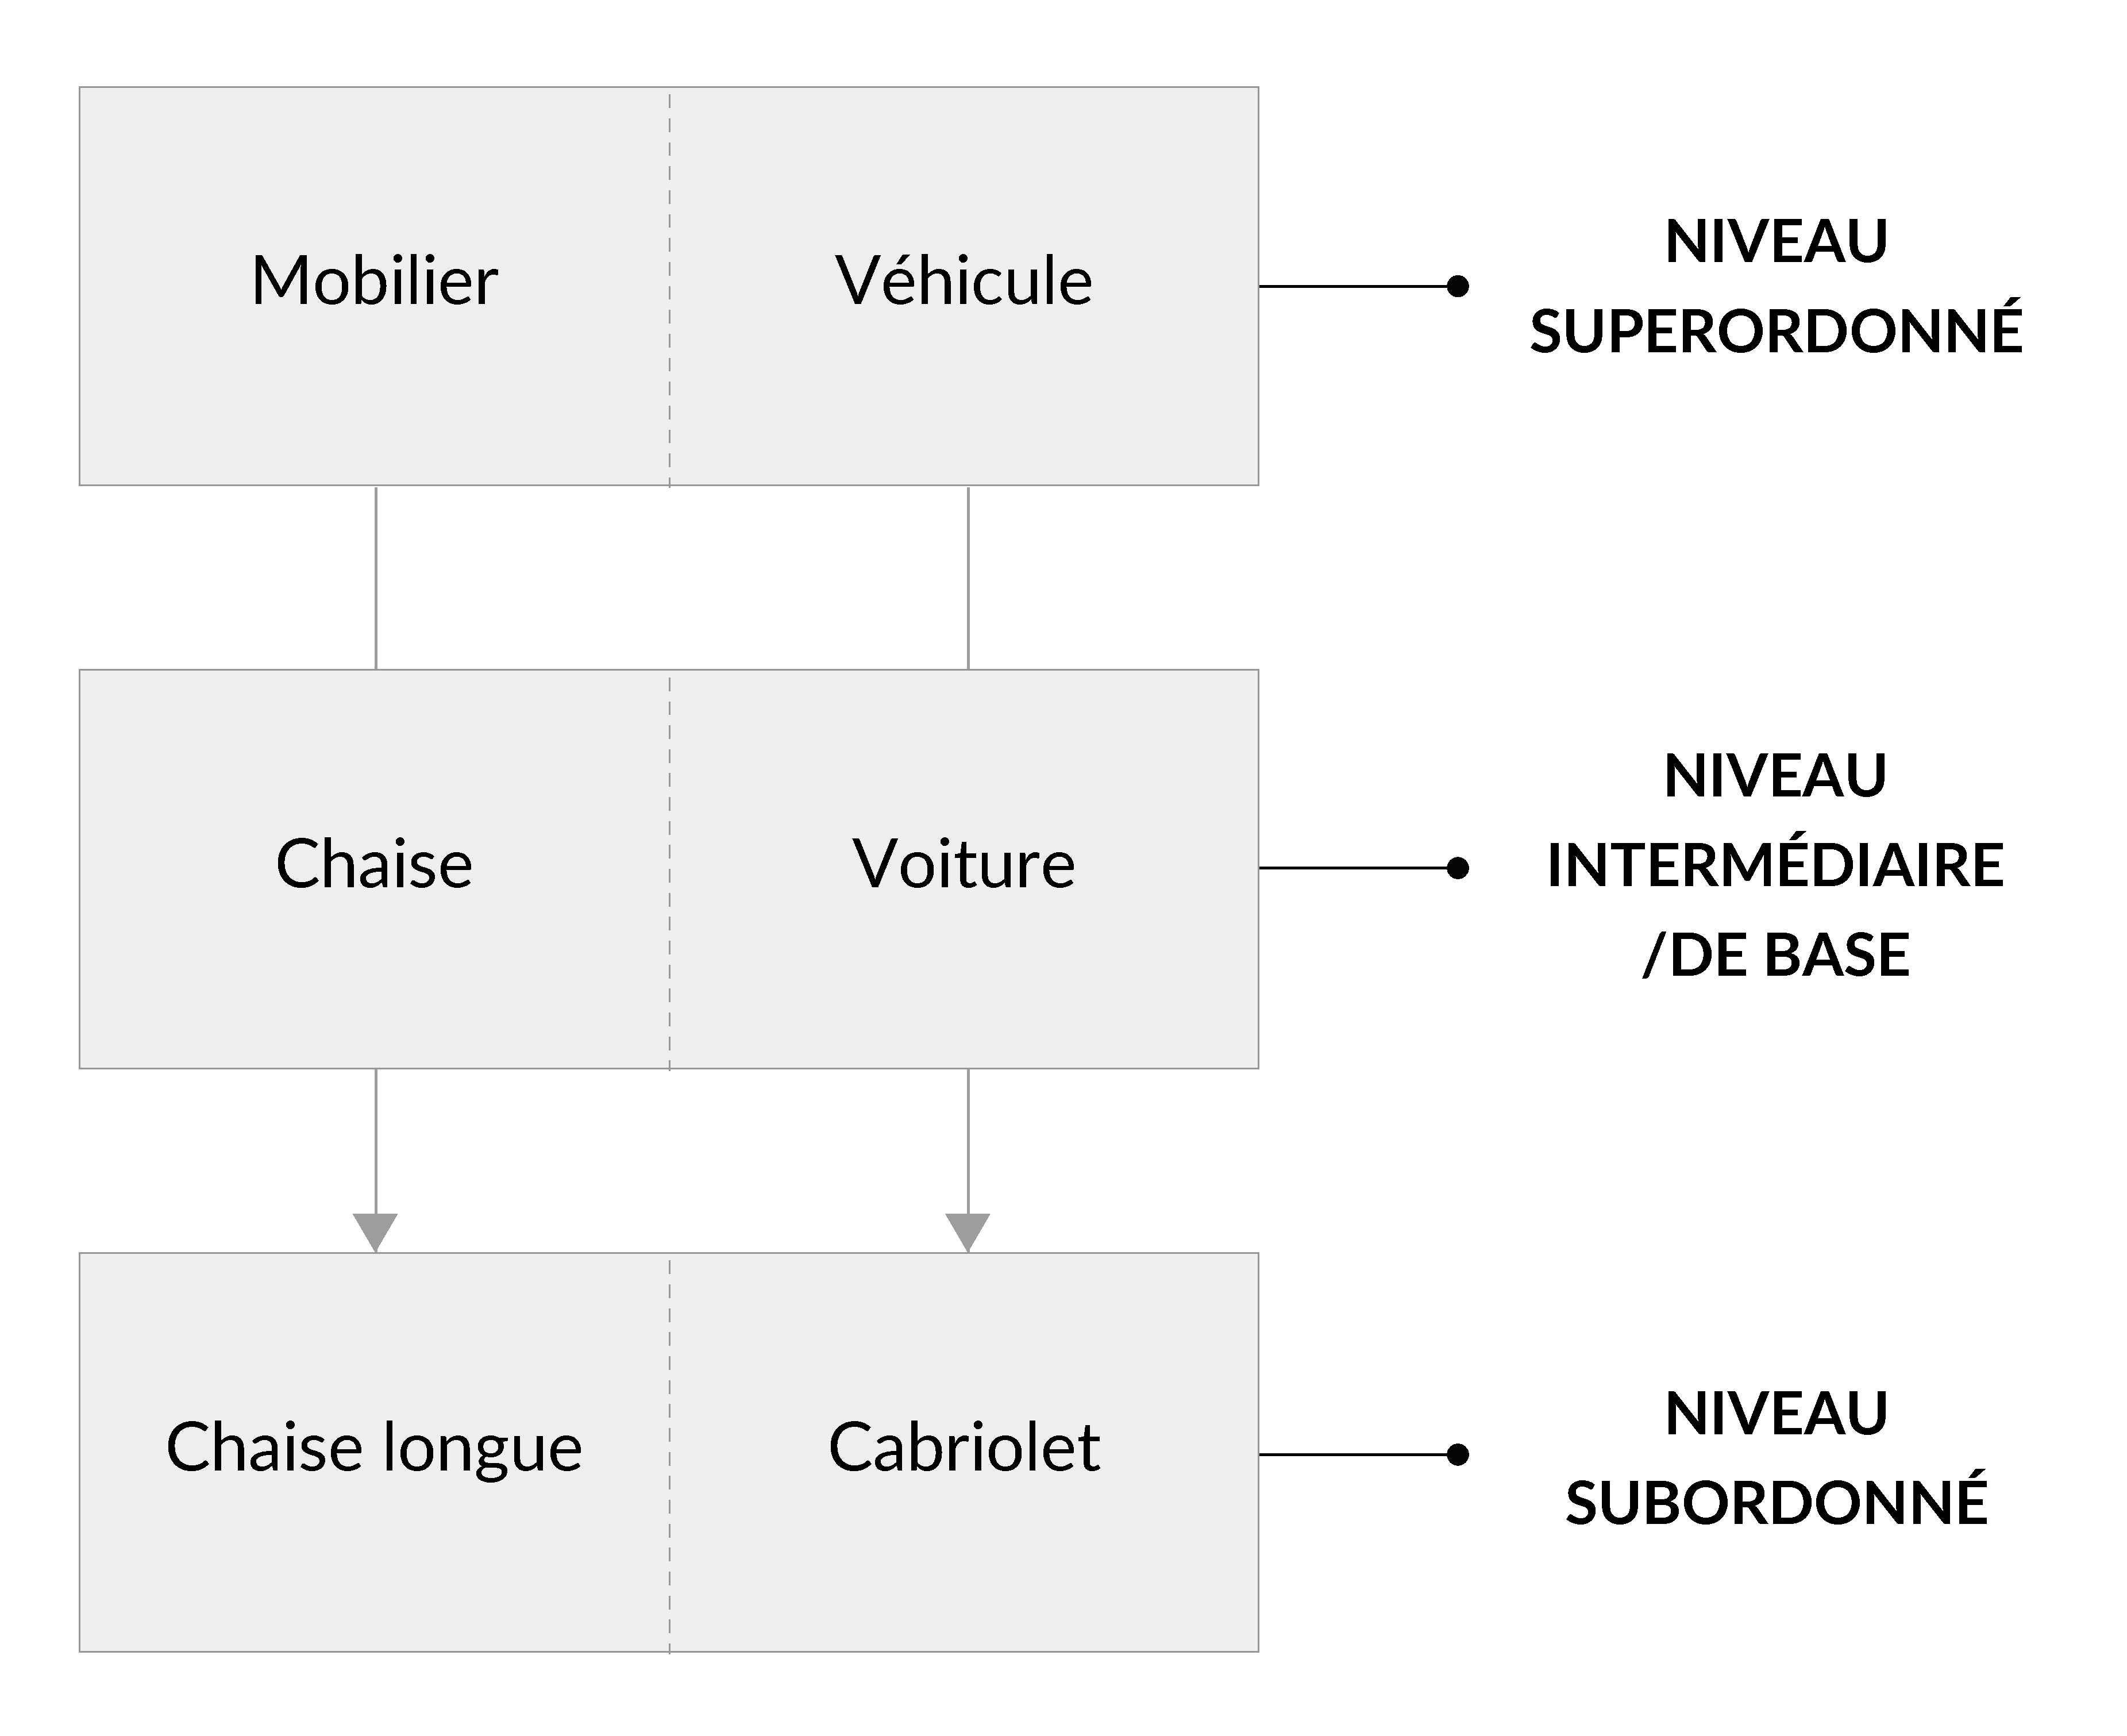
\includegraphics[width=.6\linewidth]{gfx/ch_3/categorieLVL}
        \caption{Les trois niveaux d'abstraction de l'axe vertical de la structure catégorielle.}\label{fig:categorieLVL}
\end{figure}

\subsubsection{La notion de typicalité}
\label{sec:ch3_typicité}

Une notion clef, dans les processus catégoriels, est la typicalité. Tous les objets d'une catégorie ne sont pas égaux. Il y a une gradation dans l'appartenance catégorielle. Certains objets, partageant les propriétés dominantes d'une catégorie, sont considérés comme très représentatifs de cette dernière. D'autres, ne partageant que peu des attributs caractéristiques de la catégorie, ont une appartenance moins marquée.

Le fait qu'il existe des objets plus typiques que d'autres est un constat empirique \citep[p. 37]{rosch1978cognition,mervis1981categorization}, établi à partir d'échelles de jugements (quel est l'objet le plus typique ?) ou au moyen d'épreuves de vérifications chronométrées (un chien est un animal: vrai ou faux ?) \citep[p. 41]{dubois1991semantique}.

La typicalité agit sur différents processus de traitement \citep[p. 51]{Houix03f,mervis1981categorization}:

\begin{itemize}
\item \emph{temps de traitement}: un objet typique est catégorisé plus rapidement qu'un objet moins typique;
\item \emph{apprentissage}: un enfant bâtit sa structure catégorielle en commençant d'abord par des objets typiques;
\item \emph{ordre mémoriel}: lorsqu'un sujet énumère les membres d'une catégorie, il commence par les membres typiques;
\item \emph{langage}: certains termes du langage courant sont directement connectés à la typicalité, ainsi, un ``\,moineau est un \emph{vrai} oiseau\,'', alors qu'un ``\,pingouin est une \emph{sorte} d'oiseau\,'' \citep{mervis1981categorization};
\item \emph{asymétrie des jugements de ressemblance}: il existe un phénomène d'attraction autour des objets typiques d'une catégorie. Si nous considérons la catégorie couleur, l’orange ressemble plus au rouge que le rouge ne ressemble à l'orange. L'asymétrie dans les processus perceptifs a été extensivement étudiée \citep{tversky1977features,krumhansl1978concerning}.\gl{TODO: préciser en quoi l'attraction implique l’asymétrie}
\end{itemize}


\subsection{Théories de la catégorisation}

\subsubsection{Théorie classique}

Suivant les principes de l'approche logique, dite aussi approche par règles, l'appartenance d'un objet à une catégorie se fait sur la base de règles. L'objet doit posséder un certain nombre de propriétés afin d'être assimilé à une catégorie. La nature de ces propriétés étant inhérentes à la catégorie.

Cette approche, qui sous-tend que tous les objets d'une catégorie doivent partager des propriétés communes, est aujourd'hui critiquée. Selon \citep{goldstone2003concepts}:

\begin{itemize}
\item l'appartenance catégorielle n'est pas figée: deux personnes peuvent catégoriser un même objet de deux manières. Qui plus est, une même personne peut modifier sa stratégie de catégorisation \citep{mccloskey1978natural};
\item les objets ne partagent pas le même degré d'appartenance: comme vu précédemment (\cf~Section~\ref{sec:ch3_typicité}), tous les objets à l'intérieur d'une catégorie ne sont pas égaux, certains étant plus typiques que d'autres.
\item il est difficile de définir des règles d'appartenance: définir des catégories comme ``\,célibataire\,'' nécessite d'élaborer des stratégies afin d'isoler les cas ``\,enfants\,'', ``\,veuf\,'' ou encore ``\,pape\,'' qui, intuitivement, n'ont rien à voir avec ``\,célibataire\,'' \gl{TODO: peu clair ?}. 
\end{itemize}

De plus, \citep[49]{Houix03f} souligne que, dans l'approche logique, les classes subordonnées héritent des règles d'appartenance des classes superordonnées, niant ainsi le fait qu'il existe des niveaux d'abstractions privilégiés. 

\subsubsection{Théorie prototypique}

Une alternative à l'approche classique, consiste à envisager la catégorie non plus comme relevant de règles, mais comme découlant, en quelque sorte, de la ressemblance ou ``\,air de famille\,'' liant ses membres \citep{ludwig1953philosophical}.

Partant de cette idée, la théorie prototypique a été formalisée par E. Rosch et B. B. Lloyd \citep{rosch1978cognition}. Dans celle-ci, la catégorie est définie par rapport aux objets qu'elle englobe, et non dans le but d'englober ces objets.

Pour discriminer les catégories, Rosch propose de ne pas raisonner en terme de frontières, mais plutôt de décrire chaque catégorie par un nombre de cas non ambigus (\emph{clear case}) \citep[p. 36]{rosch1978cognition}. Tous les objets d'une catégorie ne sont pas également représentatifs de cette dernière. Il a été montré que des sujets peuvent très bien s'accorder sur la typicalité d'un objet par rapport à une catégorie, tout en n'étant pas d'accord sur les frontières de cette dernière \citep{rosch1974human,rosch1975cognitive}. Les cas non ambigus peuvent être vus comme les objets les plus typiques de la catégorie. Le terme prototype, qui donne son nom à la théorie, vient de l'assertion que, parmi ces cas non ambigus, il en existe un, le prototype, plus représentatif que les autres, et qui forme le noyau de la catégorie.

Les catégories sont structurées en interne, en référence à un prototype, \ie~l'objet possédant les attributs typiques de celle-ci. L'appartenance d'un objet à une catégorie dépend alors de la ressemblance qu'entretient ce dernier avec le prototype.  Plusieurs propositions ont été faites afin de définir le prototype d'une catégorie: Pour Tversky \citep{tversky1977features}, l'élément prototype est celui dont la somme des similarités avec les autres éléments de la catégorie est la plus élevée. Pour \citep{rosch1975family}, il s'agit de l'objet possédant le plus de propriétés en commun avec les objets de la catégorie, et le moins de propriétés avec les objets des catégories externes. La typicalité d'un élément d'une catégorie s'évalue à la fois en fonction de son degré d'appartenance à celle-ci, et de son degré de différenciation vis à vis des autres catégories. 

Toutes ces approches supposent que le prototype est la représentation mentale d'un objet réel. Cependant, le prototype peut être aussi vu comme un objet stéréotypé, un assemblage des attributs les plus représentatifs de la catégorie. Ainsi, en se limitant à l'observation d'attributs vivant dans un espace métrique, \citep{reed1972pattern, rosch1976structural} ont montré que le prototype est un centroïde, un objet défini comme étant la moyenne des attributs des objets de la catégories. \gl{TODO: Préciser qu'on retrouve cette différence entre le centroïde et le medoïde}

Cette théorie prototypique de la catégorisation, bien que se basant sur des faits expérimentaux, est avant tout une vision pratique, un concept qui n'a pas été clairement défini et dont l'implication dans les processus de catégorisation reste floue \citep[p. 36-40]{rosch1978cognition} \citep[p. 49-54]{dubois1991semantique}.

\subsubsection{Théorie des exemplaires}

La théorie des exemplaires nie l'existence d'un prototype. Au contraire, elle propose que la catégorie soit représentée sur la base de tous les objets (exemplaires) la constituant, en tenant compte de leurs degrés de typicalité respectifs \citep{medin1978context,nosofsky1986attention,nosofsky1992similarity}. Ainsi, les mécanismes déductifs (\cf~Section~\ref{sec:ch3_categoPred}) peuvent profiter de tous les exemplaires de la catégorie afin d'inférer les propriétés des objets perçus. En analyse automatique, la philosophie de l'approche par les exemplaires est proche de celle des cartes auto-organisées (\emph{Self organized map}) \citep{kohonen1995som}, l’organisation du réseau et de ses nœuds étant réactualisée en fonction des propriétés de tous les items.

Plusieurs versions de cette théorie existent, entre autres, le modèle de contexte \citep{medin1978context}, et le modèle de contexte généralisé \citep{nosofsky1986attention}. Dans le modèle de contexte, les objets sont représentés suivant leurs attributs, la dimension de l'espace de représentation étant alors égale aux nombres d'attributs, choisis dans un contexte particulier \citep{hitzman1986schema}. Dans le modèle généralisé, les objets sont représentés dans un espace psychologique aux dimensions réduites, espace établi sur la base des distances inter-objets \citep{nosofsky1992similarity}. Typiquement, le positionnement multidimensionnel (\emph{multidimensional scaling}: \cf~annexe~\ref{app:mds}) est utilisé afin de reconstruire de tels espaces.

Dans la théorie des exemplaires, l'appartenance catégorielle se fait sur la base de la somme pondérée des similarités entre l'objet à catégoriser, et les exemplaires de la catégorie. Dans le modèle de contexte, la pondération s'effectue sur les propriétés des objets, et rend compte d'un poids attentionnel, favorisant les propriétés saillantes dans un contexte donné. Dans le modèle généralisé, la pondération se fait en fonction de la distance entre les exemplaires et l’objet, et ce afin de favoriser les exemplaires proches de l'objet à catégoriser.

L'approche par les exemplaires lève cependant deux questions \citep{goldstone2003concepts}:

\begin{itemize}
\item Comment justifier que nombres d'études montrent que l'appartenance catégorielle s'effectue via une comparaison à un prototype ?
\item Comment justifier que le principe d'économie cognitive reste valide, si le cerveau utilise l'ensemble des items d'une catégorie pour la représenter ? 
\end{itemize}

Dans la théorie des exemplaires, la proximité entre un objet et une catégorie est la somme des similarités entretenues entre l'objet et les items de la catégorie \citep{nosofsky1986attention}. Dans certains cas, cette opération équivaut à calculer la similarité entre l'objet et le représentant moyen des items de la catégorie. L’existence d'un prototype n'est alors qu'un artefact. Notons quand même que la théorie des exemplaires ne nie pas l'existence d'un gradient de typicalité entre les objets d'une catégorie.

Bien qu'on puisse montrer, dans le cas d'un bruit blanc, que le cerveau peut stocker en mémoire la totalité d'un signal sur une période de plusieurs semaines  \citep{agus2010rapid}, il est écologiquement peu probable que, pour chaque catégorie, le cerveau sauvegarde la totalité des exemplaires. Deux phénomènes peuvent alors intervenir: soit il existe un processus de sélection des exemplaires \citep{palmeri1995recognition}, soit les exemplaires émanant d'une même entité physique (deux exemples de pigeon), sont résumés par un même représentant \citep{barsalou1998basing} \gl{TODO: à nuancer, ces deux options sont triviales et les processus de mémorisation sont plus complexes}.

\subsubsection{Théorie des frontières}

En opposition directe avec le modèle prototypique, la théorie des frontières représente les catégories par leur périphérie. L'importance des frontières est un fait expérimental mis en avant par plusieurs études. Notamment \citep{davis2010memory} qui montre que, dans le cas de deux catégories proches, l'objet représentatif putatif n'est pas le prototype, mais une caricature de ce dernier. La caricature du prototype est une entité dont les propriétés ont été distordues afin qu'elle s'éloigne de la frontière séparant les deux catégories, distorsion qui peut substantiellement éloigner la caricature des objets de sa catégorie (\cf~Figure~\ref{fig:prototypeCaricature}).

\citep{goldstone2003concepts} souligne que les théories du prototype et des frontières peuvent se compléter: pour des catégories très éloignées, la distance au prototype (représentant moyen des objets d'une catégorie) est une information suffisante pour associer l'objet à une catégorie. Pour des catégories très similaires, l’appartenance catégorielle, afin d'être efficace, doit s'appuyer sur une information plus spécifique, à savoir la frontière.

Par ailleurs, la théorie des frontières n'envisage pas la périphérie d'une catégorie comme quelque chose de statique. Il existe une frontière a priori, certes, mais cette dernière peut bouger en fonction du contexte.

\begin{figure}[t]
        \myfloatalign
        \includegraphics[width=.8\linewidth]{gfx/ch_3/prototypeCaricature}
        \caption[Prototype et caricature]{Prototype et caricature, d'après \citep{davis2010memory}}\label{fig:prototypeCaricature}
\end{figure}


\subsection{Catégorisation et contexte sensoriel}
\label{sec:ch3_categoEtContexte}

\gl{La catégorisation d'un objet est dépendante de l'environnement dans lequel ce dernier est entendu, autrement dit des autres sons co-occurrant. Cependant la manière dont ce contexte environnemental influe sur l'identification reste méconnue.}
\jls{la catégorisation d'un objet est dépendante de l'environnement dans lequel il est perçu, c'est à dire des sons co-occurants. La manière dont le contexte influe sur l'identification est cependant méconnue.}
\gl{\citep{ballas1987interpreting} propose de voir l'environnement sonore comme une forme de langage à part entière. Comme pour la parole, les propriétés sémantiques des sons, à savoir la nature perçue de la source émettrice (\emph{trafic}, \emph{humain}, \etc), mais aussi la manière avec laquelle cette source s'accorde avec les autres sons présents, influent significativement sur leur perception. Pour la parole, il est connu que le contexte grammatical ainsi que le contexte sémantique (ici le sens de la phrase) ont un effet bénéfique sur la reconnaissance d'un mot \citep{bilger1984standardization}. \jlv{En allant au bout du parallèle entre environnement et parole} \jls{Au terme de leur comparaison}, les auteurs concluent que la source d'un son est plus facilement identifiable, si ce dernier est en adéquation avec son contexte environnemental (\eg~identifier un \emph{oiseau} dans un environnement de \emph{parc}).}

Dans \citep{ballas1991effects}, les auteurs montrent que l'effet du contexte est suppressif, à savoir qu'un contexte inadéquat a tendance à diminuer la capacité d'un individu à identifier un son, \jlc{exit: comparé au cas où le son est entendu de manière isolée}. \jlc{exit: "Aucun effet bénéfique n'est cependant observé pour un contexte adéquat". Je ne comprends pas le sens de cette dernière phrase. Est-ce bien le mot bénéfique que tu voulais employer ?.}
\jls{Dans \citep{ballas1991effects}, ils montrent même que l'effet du contexte est suppressif, à savoir qu'un contexte inadéquat a tendance à diminuer la capacité d'un individu à identifier un son.}

\gl{En appliquant ces idées à la détection automatique d'événements sonores, \citep{niessen2008disambiguating} montrent que la modélisation du contexte environnemental, \ie~la probabilité d'entendre un événement dans un type d'environnement donné et \emph{a fortiori} la probabilité de co-occurrence des événements, permet d'améliorer les performances de détection.} 

\gl{Cependant, il existe aussi des preuves montrant le phénomène inverse \jls{Le fait est, cependant, que l'inverse a aussi été prouvé...}, \ie~que le caractère incongru d'un son par rapport à son environnement peut faciliter son identification. Dans une étude approfondie, \citep{gygi2011incongruency} mettent en évidence que la source d'un événement est plus facilement identifiable, si ce dernier apparaît dans un environnement où il n'est pas ``\,censé\,'' apparaître. Il est ainsi plus facile d'isoler et identifier un son de canard dans un aéroport, qu'un son d'avion. Les auteurs appellent ce phénomène : ``\,l'Avantage de l'Incongrue\,'' (AI). Ils montrent par ailleurs que l'AI dépend du rapport entre le niveau de l'événement, et celui du fond sonore (\emph{background}). Il n'opère pas pour des rapports inférieurs à -7.5$dB$, et son effet est constant pour des rapports supérieurs à ce seuil.}

\gl{L'effet de l'AI a aussi été mis en évidence dans une étude pilote, menée dans le cadre de cette thèse, et présentée en annexe~\ref{app:xp_congruence}. Cette étude tend à montrer que l'AI dépend également de la structure temporelle de l'environnement.}
\jls{Une étude menée dans le cadre de cette thèse tend à montrer que L'AI dépend également de la structure temporelle de l'environnement. Elle est présentée en annexe~\ref{app:xp_congruence}.}
\gl{TODO: a compléter, notamment sur le lien entre environnement et parole.}

\subsection{Similarité et catégorisation}

\gl{Comme nous l'avons vu, et particulièrement dans le cas des théories prototypiques, d'exemplaires et de frontières, similarité et catégorisation apparaissent comme des concepts très proches, la catégorie étant un groupement d'objets similaires au sens de l'individu réalisant le groupement.}
\jls{Comme vu précédemment, notamment au moment d'évoquer les théories prototypiques, d'exemplaires et de frontières, similarité et catégorisation apparaissent comme des concepts très proches, la catégorie étant un groupement d'objets similaires pour l'individu réalisant le groupement.}
\gl{Les ressemblances entretenues par les objets d'une même catégorie sont globales, convoquant à la fois les propriétés physiques de ces deniers, mais également leurs propriétés sémantiques et affectives, toutes deux relatives à la connaissance de l'individu. De plus, le processus de catégorisation est lui même lié à un contexte, \jlv{"se devant de répondre aux besoin d'une situation particulière"} \jlc{là tu n'es pas clair. Il faut reformuler}, comme c'est notamment le cas pour les catégories \emph{ad hoc}.}   
\jls{Les ressemblances entretenues par les objets d'une même catégorie sont globales, liées à la fois aux propriétés physiques desdits objets, mais également à leurs propriétés sémantiques et affectives, ces dernières relevant de la connaissance de l'individu. De plus, le processus de catégorisation est lui même lié à un contexte, ..., comme c'est notamment le cas pour les catégories \emph{ad hoc}}
\gl{La similarité, quant à elle, est habituellement comprise comme une notion beaucoup plus stable, n'impliquant que la comparaison des propriétés intrinsèques des objets (forme, taille, fréquence, durée~\etc). Cependant, il faut noter que la similarité, comme la catégorisation (\cf~Section~\ref{sec:ch3_categoEtContexte}), dépendent également d'un contexte sensoriel d'exposition, \ie~du nombre et de la nature des objets présents lors de la mesure. \citep{tversky1977features,tversky1978studies} ont montré que les propriétés physiques rentrant en compte dans les mesures de similarités diffèrent suivant la diversité du corpus d'objets étudiés.}

\gl{On fait donc la distinction entre ces deux mécanismes, la similarité apparaissant comme un processus dirigé par les données (stimuli), alors que la catégorisation est elle dirigée par les connaissances de l'individu \citep[p. 59]{Houix03f}. Il est néanmoins possible de réunir ces deux notions en considérant la similarité comme un des mécanismes (essentiel) du processus de catégorisation \citep[p. 61-65]{Houix03f}.}

\section{Analyse de scènes acoustiques}
\label{sec:ch3_ASA}

\gl{TODO: plus insister sur la notion de flux, lien chapitre 4}

\subsection{Définition}
\label{sec:ASAintro}

L'analyse de scène est un procédé issu de la recherche dans le domaine de la vision, où les études portent notamment sur les stratégies suivies par l'ordinateur pour parvenir à isoler un(des) objet(s), ou une structure, d'une image~\citep[p. 12]{mcadams1994penser}. Dans le domaine de l'audition, un procédé analogue est appelé Analyse de Scène Acoustique. L'ASA a été introduite par A. S. Bregman dans son ouvrage de référence \citep{bregman1994auditory}.

L'ASA désigne l'ensemble des traitements perceptifs permettant d'isoler, dans une mixture sonore, les informations émanant de sources distinctes, et de les ``\,organiser\,'' en un tout cohérent. Ces regroupements sont nécessaires au cerveau, et donc au sujet, pour comprendre, pour donner sens à l'environnement. On parle de processus de ségrégation ou de processus de groupement \citep{winkler2009modeling}. Comme vu à la section~\ref{sec:chaineTaite}, ces processus mobilisent à la fois les traitements ascendants ou \emph{bottom-up}, intervenant au niveau de l'information auditive transduite, et les traitements descendants ou \emph{top-down}, intervenant au niveau du bagage mémoriel. Les processus \emph{bottom-up} sont appelés ``\,processus primitifs\,'', et les processus  \emph{top-down}, ``\,processus basés sur des schémas\,''. 

Les processus primitifs sont innés, et opèrent à partir des régularités du signal, afin d'en regrouper les composantes fréquentielles produites par une même source. Le mot régularité désigne ici les propriétés constantes de l'environnement, perçues par tous les individus, et en tous lieux.

Les processus basés sur des schémas sont, eux, conditionnés, et opèrent sur la base de connaissances, ou schémas, partie intégrante de notre représentation mentale du monde, représentation construite à partir des écoutes antérieures. 
\jls{Les processus basés sur des schémas sont, eux, conditionnés, et opèrent sur la base de connaissances (schémas) issues de notre représentation mentale du monde, représentation construite à partir des écoutes antérieures.}
\subsection{Une approche psychoacoustique}

Si la plupart des recherches sur l'ASA adoptent une approche cognitiviste, se concentrant sur l'étude des \emph{processus primitifs}, elles suivent généralement une méthodologie expérimentale très inspirée de la psychoacoustique. De fait, les sujets sont soumis à des stimuli décrits analytiquement dans un espace multidimensionnel de dimensions physiques (fréquence, intensité, \etc) \citep{dubois2006cognitive}. Dans la majorité des cas, ces stimuli, ou sons, qu'ils soient purs ou qu'ils soient complexes,\footnote{Un son pur est un son composé d'une seule sinusoïde, \ie~possédant une seule fréquence. Un son complexe est, lui, composé de plusieurs composantes fréquentielles} sont synthétisés en laboratoire.

Ces sons sont émis de manière séquentielle. Au cours de l'expérience, les paramètres d'écoute sont modifiés (intensité, fréquence, espace entre les séquences...) afin d'évaluer le seuil à partir duquel la capacité du sujet à distinguer les sources sonores est altérée.

L'ASA \gl{se focalise donc sur} l'analyse de l'effet de descripteurs ``\,bas niveau\,'' dans le processus d'intégration, sans tenir compte d'attributs perceptifs ``\,haut niveau\,'', comme la valeur sémantique attribuée aux sons, sans tenir compte non plus de considérations écologiques (\cf~Section~\ref{sec:ch3_ecologique}). Il est difficile de faire un parallèle entre la notion de source sonore utilisée dans le domaine de la psychoacoustique, et celle admise dans le domaine de la psychologie cognitive. Dans l'une et l'autre approche, a priori, le terme source sonore s'applique à l'objet source (\eg~voiture). C'est évident en psychologie cognitive, où le stimulus est le plus souvent un enregistrement de ladite source. Cela l'est moins en psychoacoustique, où le stimulus, synthétisé, est un objet abstrait (agglomérat de sinusoïdes), éloigné de la réalité des phénomènes acoustiques, et dont l'existence n'est avérée que dans la mesure où il est interprété par le sujet comme un tout, une entité. Les résultats obtenus à partir de ces stimuli sont difficiles à généraliser à des applications plus incarnées.

\subsection{Régularités et processus primitifs}
\label{sec:ch3_regularitesEtProcessusPrimitifs}

\begin{figure}[t]
        \myfloatalign
        \subfloat[]
        {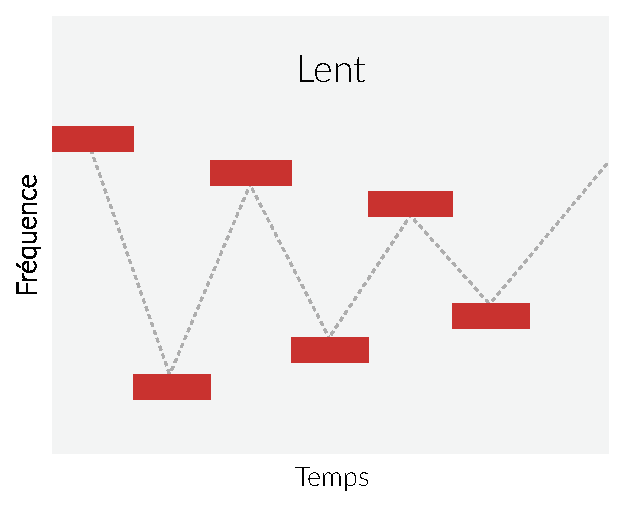
\includegraphics[width=.5\linewidth]{gfx/ch_3/tonesim_slow}}
        \subfloat[]
        {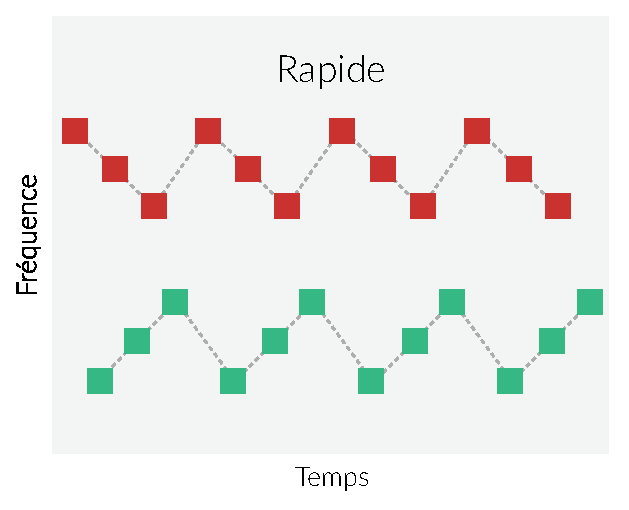
\includegraphics[width=.5\linewidth]{gfx/ch_3/tonesim_fast}}
        \caption[Groupement séquentiel : proximité temporelle.]{Groupement séquentiel: proximité temporelle. Dans l'exemple (a), la durée entre les événements est importante, aucun groupement n'est effectué, les sons sont perçus comme des événements distincts. Dans l'exmple (b) la durée entre les événements est réduite, un groupement s'opère suivant la proximité fréquentielle. Deux flux sont ainsi créés, le premier (rouge) regroupe les sons haute fréquence, le deuxième (vert), les sons basse fréquence.}\label{fig:tonesim}
\end{figure}

\begin{figure}[t]
        \myfloatalign
        \subfloat[]
        {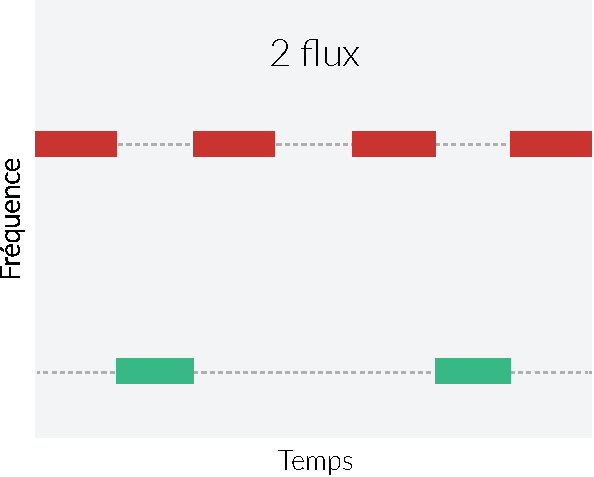
\includegraphics[width=.5\linewidth]{gfx/ch_3/gallop_2flux}}
        \subfloat[]
        {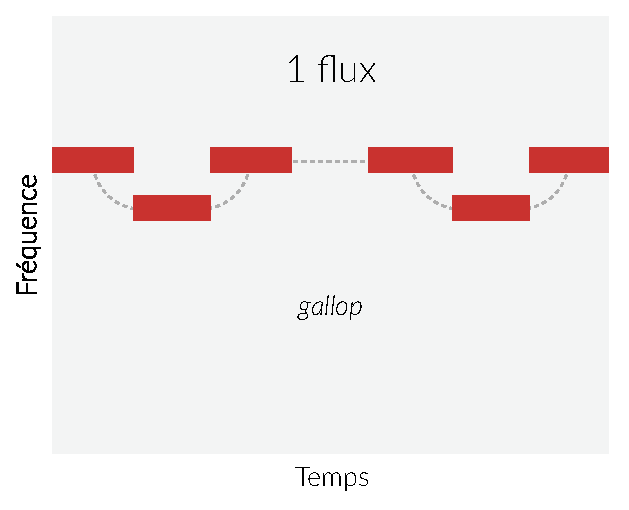
\includegraphics[width=.5\linewidth]{gfx/ch_3/gallop_1flux}}
        \caption[Groupement séquentiel : proximité fréquentielle.]{Groupement séquentiel: proximité fréquentielle. Deux groupes de sons sont joués à deux fréquences. Dans l'exemple (a), la distance entre les fréquences des sons est importante, deux flux sont créés, le premier (rouge) regroupe les sons haute fréquence, et le deuxième (vert), les sons basse fréquence. Dans l'exemple (b) la distance entre les fréquences est réduite, un groupement s'opère suivant la proximité fréquentielle. Un seul flux est créé, et l'on perçoit un motif temporel, ici, le galop d'un cheval.}\label{fig:galop}
\end{figure}

L'existence des \emph{processus primitifs} est une conséquence de l'efficience, dans le monde sonore, de régularités universelles affectant l'ensemble des stimuli auditifs. Bregman distingue 4 types de régularités [p. 19,21,31,33]\citep{mcadams1994penser}:

\begin{enumerate}
\item \emph{synchronicité}: il est rare que des sons n'ayant aucun rapport entre eux démarrent et s'arrêtent au même moment;
\item \emph{continuité}: 
\begin{itemize}
\item les propriétés d'un son isolé tendent à se modifier lentement et de façon continue;
\item les propriétés d'une séquence de sons émis par la même source tendent à se modifier lentement.
\end{itemize}
\item \emph{harmonicité}: lorsqu'un corps sonore vibre à une période répétée, ses vibrations donnent naissance à un motif acoustique dont les fréquences des composants sont des multiples d'une même fréquence fondamentale;
\item \emph{uniformité}: la plupart des modifications qui surviennent dans un signal acoustique affectent tous les composants du son résultant, de manière identique, et simultanée.
\end{enumerate}

Notre perception du monde est assujettie à ces régularités. 
Les \emph{processus primitifs}, sensibles aux stimuli exclusivement, nous permettent d'isoler du monde sonore des objets cohérents, perçus à travers elles \citep{ballas1987interpreting}. Le fait est qu'un principe similaire de perception des formes s'applique également au domaine de la vision.

\subsection{Perception de la forme}

\begin{figure}[t]
        \myfloatalign
        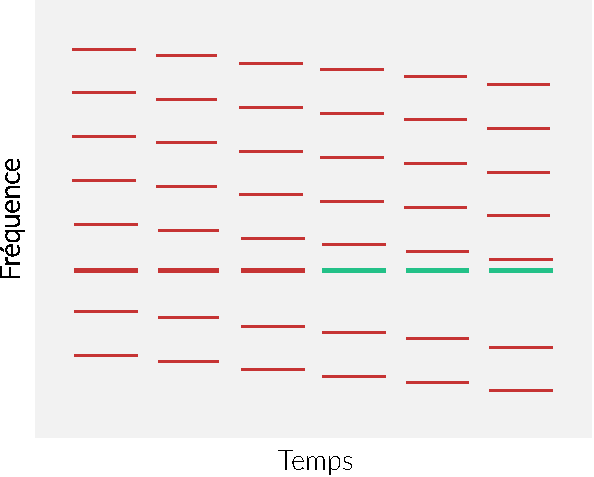
\includegraphics[width=.5\linewidth]{gfx/ch_3/harmo}
        \caption[Groupement simultané : régularité harmonique]{Groupement simultané : régularité harmonique. Un son complexe est joué plusieurs fois. A chaque occurence, on abaisse les hauteurs de la fréquence fondamentale et des harmoniques, de manière uniforme. Un harmonique est conservé à fréquence constante (trait gras). Au début, un flux est créé, \ie~les harmoniques et la fréquence fondamentale sont perçus comme étant un seul objet. Au fur et à mesure que la régularité harmonique est brisée, le cerveau tend à percevoir l'harmonique à fréquence constante dans un flux séparé, \ie~comme étant un second objet.}\label{fig:harmo}
\end{figure}

\begin{figure}[t]
        \myfloatalign
        \subfloat[]
        {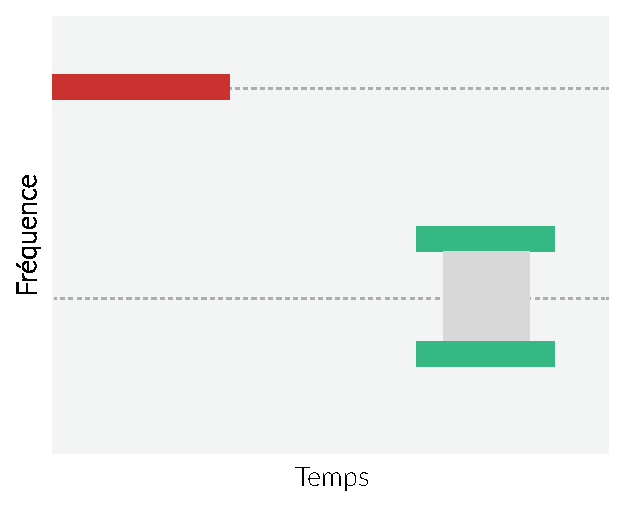
\includegraphics[width=.5\linewidth]{gfx/ch_3/opn1}}
        \subfloat[]
        {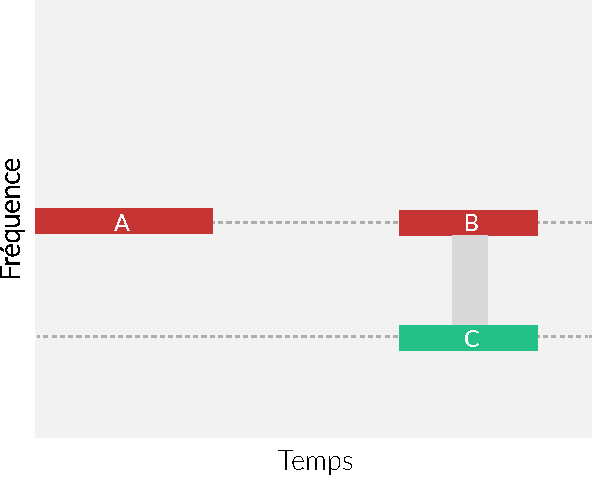
\includegraphics[width=.5\linewidth]{gfx/ch_3/opn2}}
        \caption[Groupement ancien-plus-nouveau]{Groupement ancien-plus-nouveau. Dans l'exemple (a), les sons A et B ont des fréquences éloignées. Le cerveau génère deux flux, le premier relatif au son A (rouge), et le deuxième comprenant les sons B et C (vert). Dans l'exemple (b), les sons A et B ont la même fréquence. Le cerveau interprète le son B comme étant une continuité du son A. L'attraction entre B et C en est réduite. Le cerveau génère toujours deux flux, le premier regoupant cette fois les sons A et B (rouge), et le deuxième le son C (vert).}\label{fig:oldplusnew}
\end{figure}

Que ce soit en vision ou en audition, notre cerveau est en permanence stimulé par une multitude de sources distinctes. Percevoir un objet dans cet agglomérat, c'est être capable d'isoler tous les signaux émis par une même source, et de les réunir en une unité perceptive cohérente.

Parmi les premiers travaux qui se sont intéressés à ces processus de groupement, on trouve la psychologie de la forme, en allemand \emph{Gestalttheorie}. Cette théorie, introduite par Ernst Mach et Christian von Ehrenfels à la fin du XIXème siècle, explicite les principes selon lesquels des stimuli sensoriels sont combinés, afin de former un pattern mental rendant compte de la présence d'un objet dans un environnement donné.

Mis en évidence en perception visuelle, ces principes restent vrais en perception auditive \citep[ch. 1]{bregman1994auditory}. Parmi ces principes, nous en détaillons ici cinq:

\begin{enumerate}
\item \emph{proximité}: des éléments proches les uns des autres ont tendance à être groupés ensemble. En audition, ce principe de proximité opère suivant les différentes caractéristiques du son, à savoir, la fréquence, l'\emph{onset} \footnote{En traitement du signal audio, on désigne par le mot anglais \emph{onset} le début du signal. Ce terme étant couramment utilisé en français, nous ne le traduirons pas dans ce document.} et l'intensité.
 
\item \emph{similarité}: des éléments qui se ressemblent ont tendance à être groupés ensemble. 

Commentaire. Dans le domaine de la vision, la proximité est une notion de spatialité. La similarité, elle, s'applique aux caractéristiques physiques de l'objet (forme, couleur, etc $\ldots$), qui ne peuvent se décrire dans une dimension unique. 

Dans le domaine de l'audition, la proximité est généralement admise comme notion de temporalité (\emph{onsets} proches). Pour le reste des descripteurs, il est cependant difficile de distinguer les principes de proximité et de similarité. Bregman propose de parler de proximité lorsqu'on traite d'une dimension physique particulière, et de parler de similarité dès lors qu'on considère un ensemble de descripteurs, ou lorsque l'on traite d'attributs qui ne peuvent être clairement décomposés suivant des dimensions distinctes. Exemple: le timbre.

\item \emph{continuité}: des éléments qui varient de manière non abrupte ont tendance à être groupés ensemble. Par ce principe, des objets distincts mais proches temporellement (en vision, proches spatialement) ont tendance à être reçus comme le prolongement des uns par les autres. C'est ce principe qui nous permet de percevoir comme une seule entité un objet dont les caractéristiques varient dans le temps, \eg~le son d'une sirène. \emph{A contrario}, un changement abrupt indique généralement l'apparition d'une nouvelle source.

De récentes études en neurosciences ont montré l'importance de ce principe dans les processus de groupement. \citep{winkler2009modeling}  propose de voir l'ASA comme un processus prédictif, le cerveau cherchant à anticiper la nature des stimuli qui lui parviennent, sur la base de régularités extraites des objets détectés dans l'instant précédant.

\item \emph{clôture}: des éléments discontinus, qui suggèrent la forme d'un objet continu, ont tendance à être groupés ensemble. De manière automatique, le cerveau tend à percevoir un ensemble d'objets distincts comme un tout. En audition, ce principe est très lié à la notion de masquage. En effet, les sons que nous percevons sont régulièrement masqués par d'autres sons concurrents, éventuellement plus forts. Le principe de clôture nous permet de compenser ce phénomène de masquage, et de percevoir le signal sans discontinuité. Ainsi lorsqu'un son pur est régulièrement entrecoupé de silences, nous percevons une série de sons purs, mais, si ces silences sont comblés par un bruit blanc, nous percevons un son pur continu. Ce phénomène est parfois appelé ``\,l’illusion de continuité\,'' \citep{dannenbring1976perceived}, et s'applique particulièrement dans le contexte de la perception de la parole \citep{carlyon2002continuity}.

\item \emph{destin commun}: des éléments qui varient de manière synchrone et uniforme ont tendance à être groupés ensemble. Comme évoqué à la section~\ref{sec:ASAintro} c'est ce principe qui permet de percevoir comme un tout les différents harmoniques qui composent un son complexe. C'est également ce principe qui nous incite à percevoir de manière unie des stimuli ayant le même \emph{onset} temporel.
\end{enumerate}

Ces principes agissent de concert afin de grouper les composantes du son en flux auditifs.

\subsection{Flux auditif et stratégie de groupement}

\begin{figure}[t]
        \myfloatalign
        \subfloat[]
        {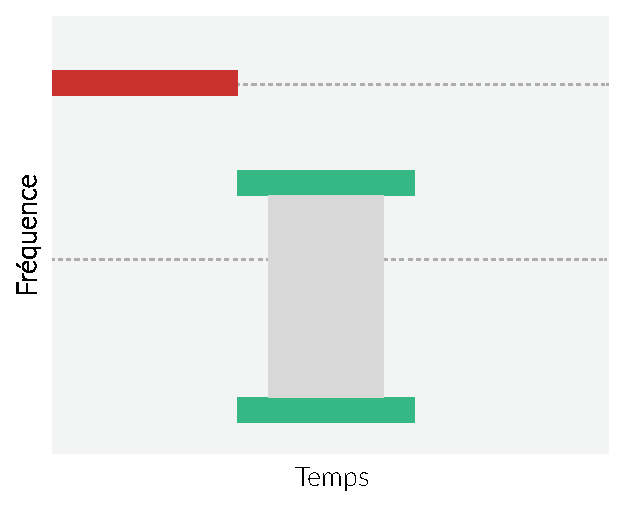
\includegraphics[width=.5\linewidth]{gfx/ch_3/seqsim1}}
        \subfloat[]
        {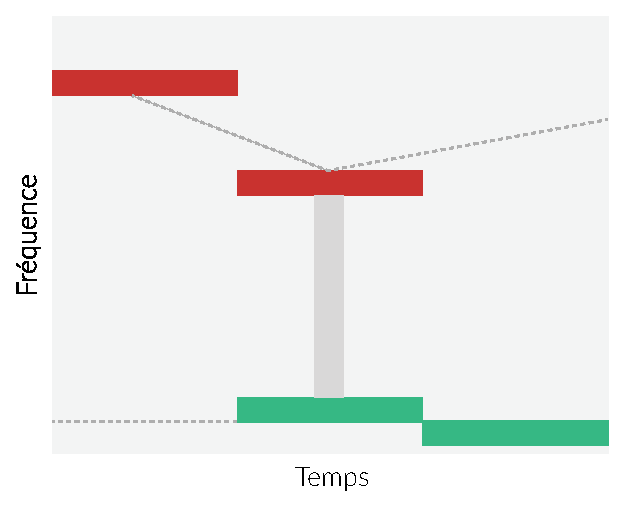
\includegraphics[width=.5\linewidth]{gfx/ch_3/seqsim2}}
        \caption[Compétition entre groupement séquentiel et groupement simultané]{Compétition entre groupement séquentiel et groupement simultané. Dans l'exemple (a), le cerveau perçoit deux flux, le premier regroupant le son A (rouge) et le deuxième regroupant les sons B et C (vert). Dans l'exemple (b), un quatrième son (D) est ajouté, ce dernier possédant une fréquence très proche de celle de (D). Le groupement sequentiel par proximité fréquentielle entre les couples A-B et C-D est favorisé, au détriment du groupement simultané entre les sons B-C.}\label{fig:simvsseq}
\end{figure}

L'une des notions les plus importantes en ASA est le concept de flux auditif (\emph{auditory stream}), que Bregman définit comme ``\,le groupement perceptif que nous faisons des parties du spectre qui vont ensemble\,''.

Contrairement au terme ``\,son\,'', qui peut faire référence aux réalités physiques des phénomènes acoustiques, aussi bien qu'aux représentations mentales que nous nous en faisons, le flux auditif désigne spécifiquement une entité perceptive.

Le terme flux se veut volontairement généraliste. Ce dernier peut désigner aussi bien un son isolé (un coup de marteau), que plusieurs sons, à condition que ces derniers soient perçus comme formant une seule entité (une série de coups de marteau rapprochés).

On désigne par ``\,formation de flux auditifs\,'' (\emph{auditory streaming}) , le processus à l'origine de la création de flux. \citep{winkler2009modeling} proposent la définition suivante en ce qui concerne la formation de flux auditifs:

\begin{quote}
``\, Un phénomène perceptif dans lequel une séquence de sons est perçue comme étant composée de deux ou plusieurs flux auditifs \,''
\end{quote}

Comme nous le voyons, le flux désigne une représentation perceptive d'un son, et, à ce titre, il est l'équivalent auditif de l'objet pour la vision \citep[p. 11]{bregman1994auditory}. Cependant, nous notons que la notion de flux, et plus particulièrement celle de formation de flux, est souvent utilisée dans un contexte où une dimension temporelle est sollicitée. On parle d'ailleurs de construction de flux (\emph{build-up of streaming}) pour désigner la période durant laquelle le cerveau accumule des indices afin de générer et stabiliser les flux auditifs  \citep{cusack2004effects,snyder2007toward}. Ainsi, dans ce document, nous réservons les termes ``\,flux\,'' pour désigner les représentations mentales des stimuli en train d'être traités (intégrés temporellement), et ``\,formation de flux auditifs\,'' pour désigner les processus perceptifs de groupement des sons. Nous conservons le mot ``\,objet\,'' pour désigner, de manière générale, les représentations mentales, stockées en mémoire, des phénomènes acoustiques.

En ce qui concerne les processus primitifs, on distingue trois stratégies de groupement:

\begin{itemize}
\item \emph{groupement séquentiel}: désigne le groupement de sons ne partageant pas un même \emph{onset}. Dans le cas de sons purs, le groupement séquentiel s'appuie beaucoup sur le principe de \emph{proximité}, et notamment de \emph{proximité} fréquentielle, principe qui veut que, plus deux sons sont proches en fréquence, plus ils ont tendance à être regroupés dans le même flux (\cf~Figure~\ref{fig:galop}). Pour des sons complexes, c'est plutôt le principe de similarité qui entre en jeux. La \emph{proximité} temporelle, \ie~la durée séparant chaque son, rentre cependant en ligne de compte. Plus cette dernière est faible, plus deux sons ont des chances d'êtres regroupés (\cf~Figure~\ref{fig:tonesim});
\item \emph{groupement simultané}: aussi appelé groupement spectral, désigne le groupement des composantes fréquentielles qui partagent un même \emph{onset}. Le groupement simultané s'appuie principalement sur la régularité harmonique. Une composante fréquentielle venant briser la suite harmonique tend à être isolée dans un autre flux auditif (\cf~Figure~\ref{fig:harmo});
\item \emph{groupement ancien-plus-nouveau}: ce groupement est l'application directe du principe de continuité. Lorsque le spectre de l'environnement sonore s'enrichit subitement, tout en conservant ses composantes fréquentielles de départ, le cerveau tend à interpréter l'ajout comme une continuation de l'ancien, et à l'intégrer dans le même flux sonore (\cf~Figure~\ref{fig:oldplusnew}).
\end{itemize}

Dans le cas d'une compétition entre un groupement séquentiel et un groupement simultané, c'est l'organisation issue du groupement séquentiel qui prime (\cf~Figure~\ref{fig:simvsseq}). Ce phénomène fait sens d'un point de vue écologique. En effet la plupart des sons, et en particulier ceux utilisés pour la communication, n'existent que dans une certaine durée, et sont intermittents. Il est alors nécessaire de faire des associations entre des sons parfois séparés par un intervalle de temps long, afin de percevoir le sens du message \citep{winkler2009modeling}.

Les exemples cités plus haut se placent tous dans un contexte \emph{bottom-up}, en évacuant d'éventuels processus attentionnels. Bien que cela ait été encore très peu étudié, il paraît cependant évident que ces stratégies de groupement s’opèrent également dans un contexte \emph{top-down}, en s'appuyant sur une mémoire à plus long terme.


\subsection{Attention, saillance et perception}

L'attention est la capacité de notre système auditif à focaliser sur des composantes spécifiques de notre environnement sonore en ignorant le reste. En fonction du contexte de la scène, certains flux ont tendance à attirer plus facilement notre ``\,attention\,''. Un des paramètres pouvant susciter l’attention est la saillance.

La saillance d’un flux audio peut se voir comme l’impact potentiel d’un stimulus sur notre perception, et notre comportement. Cette saillance est fonction du contexte d'écoute de la scène sonore. L’attention et la saillance ont une influence dans l’identification des sources. Cette identification, et l'attribution de ``\,sens\,'' qui en découle, est une étape primordiale dans le processus de création de l’image mentale d’un environnement, à partir de la perception de son empreinte sonore. Ainsi, un élément saillant est facilement identifiable. A l'inverse, les sources d'un fond sonore (\emph{background}), par définition peu saillant (\ie~attirant potentiellement moins l’attention), seront moins discernables \citep{elhilali2009interaction}.

De Coensel et Botteldooren proposent plusieurs modèles permettant de simuler l’attention \citep{botteldooren2009role,de2010model,de2010application}. Les modèles calculent une ``\,carte de saillance\,'' décrivant l’évolution de la saillance d’une scène en fonction du temps. Les deux chercheurs partent du principe que le cerveau ne peut pas traiter toutes les informations en même temps. Il sélectionne l'information utile. Ces modèles ne prennent cependant pas en compte les traitements de type \emph{top-down} et se concentrent sur les processus \emph{bottom-up} relatifs à l’analyse des caractéristiques propres aux stimuli.

Ce modèle d'attention a été inclus dans un modèle plus général permettant de détecter les sources sonores actives dans un environnement \citep{oldoni2012computational,oldoni2013computational}. Ce modèle permet, entre autre, de composer des résumés acoustiques des environnements sonores, à partir des sons sons jugés typiques de ces derniers.

\subsection{L'approche par les neurosciences}

\gl{TODO: review \citep{snyder2007toward}}

\section{L'étude des paysages sonores}
\label{sec:paysageSonore}

\subsection{La notion de paysage sonore}

La notion de paysage sonore (\emph{soundscape}) a été introduite par Schafer dans les années soixante-dix dans son livre \citep{schafer1969new}, et détaillée dans l'ouvrage de référence \citep{schafer1977tuning}. La question que pose Schafer est:

\begin{quote}
``\,Quelle est la relation entre l'homme et les sons de l'environnement qui est le sien, et que se produit-il lorsque ces sons viennent à changer ?\,''
\end{quote}

Une première définition du paysage sonore a été donnée par \citep{truax1978handbook}:

\begin{quote}
``\,[a]n environment of sound (or sonic environment) with emphasis on the way it is perceived and understood by the individual, or by a society.\,'' 
\end{quote}

Aujourd'hui, cependant, on s'accorde sur la définition suivante \citep{aletta2016soundscape}:

\begin{quote}
``\,Un environnement sonore tel qu'il est perçu, expérimenté et/ou compris par un individu ou une communauté, dans son contexte.\,'' \footnote{Cette définition a été publiée dans le cadre de la norme \emph{ISO-12913} \citep{iso12913}}
\end{quote}

L'une et l'autre définition sont larges. Tout environnement peut être considéré comme un paysage sonore dès lors qu'on lui associe un ensemble de sons entendus par un sujet donné. Le problème est d'envisager l’environnement sonore par rapport à l'évaluation subjective de l'auditeur, et non uniquement par rapport à ses paramètres acoustiques. Schafer, déjà, explique la nécessité de ne plus considérer le bruit seul, mais aussi la perception de ce bruit par les individus, et le contexte dans lequel il est perçu, ceci afin d'améliorer la qualité de leur environnement. On parle d'environnement sonore lorsqu'on se réfère au phénomène acoustique physique, et de paysage sonore lorsqu'on se réfère à la représentation que l'on se fait de l'environnement.

Ainsi, les études sur les paysages sonores suivent le paradigme de la psychologie cognitive \citep{dubois2006cognitive,maffiolo_caracterisation_1999} (\cf~Section~\ref{sec:ch3_psychoCog}). L'environnement sonore est décrit en utilisant à la fois des descripteurs acoustiques (mesures), et des descripteurs perceptifs, l'analyse de l'interaction entre ces descripteurs permettant de comprendre les processus cognitifs mis en œuvre dans l'évaluation perceptive des paysages sonores.

L'approche étant ainsi centrée sur le sujet, les recherches sur les paysages sonores sont par essence interdisciplinaires \citep{davies2013perception,aletta2016soundscape}, faisant appel à des outils et des méthodes provenant de champs de recherches variés comme l'acoustique, la psychologie cognitive, la psycho-linguistique, la sociologie, et plus récemment, l’intelligence artificielle.

\subsection{Application à la nuisance sonore urbaine}
\label{sec:ch3_urbanNoiseSoundscape}

La ville est un environnement bruyant. Elle l'a été de tous temps. Déjà dans les rues de la Rome antique, le bruit des chariots pose problème\footnote{\cf~Juvenal, Satire 3.232–238}. Le consul Jules César interdit d'ailleurs à ces derniers de circuler la nuit. Ce qui a changé, par contre, c'est la perception du bruit. Dans les années 70-80, le bruit ``\,devient\,'' pollution, facteur de dégradation de la qualité de vie. Cette pollution est d'autant plus critique que d'ici 2050, 68\% de la population mondiale sera urbaine \citep{park14}.

Les chercheurs se concentrent alors sur l'identification des sources du bruit, et sur les moyens d'abaisser les niveaux sonores. Les premières législations anti-bruit apparaissent, qui proposent/imposent une réduction du niveau des bruits produits, essentiellement, par les transports et l'industrie.

Mais le problème persiste, le bruit demeurant un phénomène subjectif, autrement dit dépendant de l'appréciation de l'auditeur. Le bruit est affaire de contexte et beaucoup de lieux urbains sont appréciés aussi pour leur atmosphère vivante, c'est à dire ``\,bruyante\,''. Ville agréable ne rime pas nécessairement avec ville silencieuse.

Corriger l'environnement sonore uniquement suivant des paramètres acoustiques, par définition objectifs, ne suffit donc pas. Il est aujourd'hui communément admis que des mesures objectives de niveaux sonores (\eg~$L_{Aeq}$) ne peuvent, seules, rendre compte du confort sonore, et que \gl{vouloir influer sur l'environnement} uniquement sur la base de paramètres acoustiques, par définition objectifs, ne suffit pas \citep{yang2005acoustic,schulte2006soundscape,kang2010semantic,aletta2016soundscape}. Il faut désormais envisager le bruit non plus seulement comme un objet physique, mais encore comme un objet cognitif \citep{guastavino_etude_2003}. Le problème n'est plus de savoir à partir de quand un son est gênant, mais pourquoi il est perçu comme tel, et par tel individu. Les recherches se sont ainsi portées sur la notion de paysage sonore, envisageant la nuisance sonore et à travers les aspects qualitatifs, et à travers les aspects sémantiques des phénomènes acoustiques.

De plus, si beaucoup d’efforts sont faits afin de réguler les niveaux de bruits des sons non-désirés, l'approche inverse, \ie~ ajouter des sons positivement connotés, reste très peu considérée. Cette approche, consistant à identifier et agir sur les sons acceptés, ou plaisants, afin d'améliorer la qualité d'un environnement, est nommée l'approche positive par Schafer. De récentes études ont donné des résultats prometteurs, notamment \citep{hong2013designing} qui montre que l'ajout de sons d'oiseaux, ou d'eau, à des sons de trafics urbain, permet de significativement améliorer l'appréciation de ces derniers. \citep{galbrun2012perceptual} montre qu'un son d'eau ayant un niveau sonore similaire ou inférieur de -3$dB$ à celui du trafic permet de correctement masquer ce dernier. L'étude indique également que des sons de cours d'eau possédant un contenu fréquentiel basse-fréquence sont préférés aux sons de fontaines et de chutes d'eaux.\\

Depuis vingt ans, l'approche par les paysages sonores a permis de développer une base de descripteurs qualitatifs et acoustiques grâce auxquels nous jugeons mieux, et sommes mieux à même d'améliorer l'environnement sonore urbain.  \citep{kang2006urban,schulte2007soundscape}

Un des enjeux actuels de l'analyse des paysages sonores est de relier ces données perceptives, établies à partir d'enquêtes, à des mesures acoustiques, afin de pouvoir établir une politique de réduction du bruit efficace, adaptée à chaque situation \citep{schulte2013soundscape}.
Cependant, le caractère pluridisciplinaire de ces recherches, et l'utilisation de protocoles expérimentaux variés pour évaluer l'environnement sonore, rendent l’intégration des résultats difficile \citep{davies2013perception}. De plus, il n'y a toujours pas de consensus sur les descripteurs (acoustiques ou perceptifs) à utiliser pour caractériser un paysage sonore \citep{brocolini2012prediction,aletta2016soundscape}, ce qui empêche la communauté, d'une part, de présenter aux décideurs des indicateurs génériques d'évaluation des paysages sonores, et d'autre part, d'élaborer/proposer des modèles crédibles sur la base de ces expertises.

Récemment, plusieurs projets internationaux ont été lancés afin de standardiser les pratiques expérimentales des recherches portant sur les paysages sonores, notamment \emph{the European Cooperation in Science and Technology Action}\footnote{TD0804: \emph{soundscape of European Cities and Landscapes}: \url{http://www.cost.eu/COST_Actions/tud/TD0804}} \citep{schulte2010soundscape} et \emph{the Positive Soundscape project} \citep{salford2106,davies2013perception}. Mais les difficultés persistent \citep{schulte2013soundscape,ribeiro2013heart}. 

Afin d'acquérir la masse de données nécessaire permettant d'évaluer la qualité de l'environnement sonore sur un temps long, les caractéristiques d'un environnement variant au cours de la journée, et suivant les saisons, \citep{park14} ont lancé un projet collaboratif d'envergure afin de déployer, à New York, un réseau de senseurs capable de capturer en continu et en temps réel, toutes les informations nécessaires afin de rendre compte de la qualité de l’environnement évalué.
\jls{Afin d'acquérir la masse de données nécessaire permettant d'évaluer la qualité de l'environnement sonore sur un temps long, les caractéristiques d'un environnement variant au cours de la journée, comme au cours des saisons, \citep{park14} ont lancé, à New York, un vaste projet collaboratif de déploiement d'un réseau de senseurs capable de capturer, en continu et en temps réel, toutes les informations relatives à la qualité de l’environnement évalué.}
\subsection{Approches catégorielle et dimensionnelle}
\label{sec:ch3_appCatDim}

Deux grandes problématiques intéressent la recherche sur les paysages sonores:

\begin{itemize}
\item la première concerne la \emph{représentation mentale des paysages sonores}. Comment nous représentons nous, en mémoire, un paysage sonore perçu ? La question en amène deux autres:

\begin{enumerate}
\item Quelles sont les différentes catégories de paysages sonores ?
\item Comment caractériser ces catégories ?\footnote{Répondre à cette dernière question revient à comprendre quels sont les éléments qui constituent un paysage sonore, et comment la nature de ces éléments influe sur le processus de catégorisation de l'environnement. Intuitivement, les éléments constitutifs d'un paysage sonore sont les sources sonores. Il s'agit alors, également, d'étudier la manière dont nous nous représentons ces sources.}
\end{enumerate}

\item la deuxième concerne les \emph{dimensions perceptives}.  Quelles \emph{dimensions perceptives} entrent en jeu dans l'évaluation subjective des paysages sonores ?  Là encore la question en amène deux autres:
\begin{enumerate}
\item Quels descripteurs perceptifs permettent de caractériser les dimensions perceptives à partir desquelles nous appréhendons l'environnement sonore ?
\item Quels indicateurs influent sur ces descripteurs perceptifs ?
\end{enumerate}

Développons. Les descripteurs perceptifs caractérisent les dimensions selon lesquelles nous interprétons l'environnement. Pour exemple, un des descripteurs perceptifs communément utilisé est l'agrément (\cf~Section~\ref{sec:descripteursPercetifs} pour plus de détails sur les descripteurs couramment utilisés). 
Un des enjeux de l'approche dimensionnelle est de trouver les indicateurs qui influent sur ces descripteurs perceptifs. On distingue quatre types d'indicateurs.

\begin{itemize}
\item \emph{indicateurs acoustiques/physiques}: il s'agit d'indicateurs objectifs, obtenus via des mesures. Parmi ces indicateurs, certains caractérisent le niveau sonore par une approche holistique ($L_{Aeq}$), d'autres par une approche statistique ($L_{A10-90}$), d'autres encore en considérant séparément les différents canaux fréquentiels. On inclut, d'autre part, dans les indicateurs acoustiques/physiques, des indicateurs permettant de décrire les caractéristiques spectrales du son (\cf~tableau~\ref{tab:acousIndi}).

\item \emph{indicateurs perceptifs}: les dimensions affectives suivant lesquelles nous percevons l'environnement sonore ne sont pas indépendantes. Ainsi certains descripteurs, comme l'agrément ou le confort, peuvent eux-mêmes servir d'indicateurs pour d'autres descripteurs plus généraux comme la qualité sonore. On inclut, d'autre part, dans les indicateurs perceptifs, des indicateurs procédant d'une évaluation subjective d'un attribut physique (\eg~niveau sonore perçu).

\item \emph{indicateurs psychoacoustiques}: ces indicateurs sont à mi-chemin entre les indicateurs acoustiques et les indicateurs perceptifs. Comme les premiers, ils sont objectifs, calculés sur le signal sonore. Comme les seconds, ils sont perceptivement inspirés, \ie~construits afin de rendre compte d'une réalité perceptive. Pour exemple, on cite la \emph{loudness} de Zwicker \citep{zwicker2013psychoacoustics} qui rend compte du niveau sonore perçu. Le tableau~\ref{tab:psychoAcousIndi} présente quelques uns des indicateurs les plus utilisés.

\item \emph{indicateurs extra-sonores}: on regroupe ici tous les indicateurs qui ne sont pas liés au son. Certains sont liés au sujet (âge, genre, humeur), d'autres aux stimuli visuels, \gl{d'autres encore au moment de la journée}. Contrairement aux indicateurs acoustiques, psychoacoustiques et perceptifs, qui sont tous évalués/mesurés suivant des échelles ordonnées, discrètes ou continues, certains indicateurs extra-sonores sont eux évalués sur des échelles de catégories\footnote{Le terme catégorie, employé pour décrire un type d'échelle, n'a rien à voir avec le terme catégorie relatif au représentations mentales} (\eg~Genre: homme/femme). On parlera alors plutôt de contexte extra-sonore.
\end{itemize}

\end{itemize}

Ces problématiques, pour rappel, la représentation mentale des paysages sonores, et les dimensions perceptives, sont à la base des deux grandes approches méthodologiques adoptées par la communauté scientifique, l'approche catégorielle, et l'approche dimensionnelle. On note cependant qu'avec le temps, la communauté privilégie l'approche dimensionnelle. \\


\begin{table}[t]
\centering
\begin{tabular}{c c} 
\multicolumn{2}{c}{Acoustique} \\ 
Nom                           & Description            \\                                                            
\hline
$L_{A}$                                   & Niveau sonore calculé      \\
                                          & avec une pondération $A$\\
$L_{Aeq}$                                 & Moyenne des $L_A$     \\
                                          &         \\
$L_{A10-90}$                              & 10-90ème quantiles des $L_A$     \\
                                          &         \\
$L_{Amin}, L_{Amax}$                      & minimum maximum des $L_A$    \\
                                          &         \\
Facteur crête                             & Ratio entre la valeur de pression     \\
                                          & maximale et la valeur $RMS$        \\                                          
\hline
\end{tabular}
\vspace{0.5mm}
\caption{\gl{TODO} Indicateurs acoustiques}
\label{tab:acousIndi}
\end{table}

\begin{table}[t]
\centering
\begin{tabular}{c c} 
\multicolumn{2}{c}{Psychoacoustiques} \\ 
Nom                           & Description            \\                      
\hline
\emph{loudness} de Zwicker                & Niveau sonore perçu     \\
                                          &         \\
Acuité (\emph{sharpness})                 & Contenu fréquentiel       \\
                                          &         \\
Rugosité (\emph{roughness})               & Modulation enveloppe        \\
                                          & temporelle (15-70Hz)       \\
Fluctuation (\emph{Fluctuation strength}) & Modulation enveloppe      \\
                                          & temporelle (4Hz)          \\
Brillance                                 & Centre de gravité       \\
                                          & spectral         \\                                       
\hline
\end{tabular}
\vspace{0.5mm}
\caption{Indicateurs psychoacoustiques: modèles mathématiques illustrant des qualités affectives perçues}
\label{tab:psychoAcousIndi}
\end{table}


\subsubsection{Méthodologie de l'approche catégorielle}
\label{sec:ch3_appCategorielle}

Les objectifs de l'approche catégorielle sont triples. Il s'agit:

\begin{itemize}
\item d'appréhender les principes psychologiques qui sous-tendent la formation des représentations mentales;
\item d'objectiver la nature de ces représentations;
\item de comprendre l'influence de ces représentations sur le traitement de l'information sonore.
\end{itemize}
 
À ce titre, l'approche catégorielle peut être vue comme une approche cognitive. 

Afin d'objectiver la nature des catégories mentales représentant des paysages sonores, ou des sources sonores, l'approche catégorielle peut avoir recourt à trois types d'expériences (\cf~Figure~\ref{fig:descat}) :

\begin{itemize}
\item \emph{Tâche de description}: On demande au sujet de décrire l'environnement sonore auquel il a été exposé \citep{axelsson2005soundscape,raimbault2005urban,guastavino2006ideal,raimbault2006qualitative}, soit de la manière la plus libre possible, soit en contraignant la description par le biais d'un questionnaire. Là encore, les réponses peuvent être libres (questionnaire semi-dirigé) ou à choix forcés (questionnaire dirigé). Plus la description est libre, plus on accède à des représentations mentales spécifiques au sujet. \emph{A contrario}, plus le questionnaire est contraint, plus on accède à des représentations stéréotypées. 

L'analyse linguistique et lexicale des données ainsi collectées permet d'en faire émerger les catégories sémantiques. La richesse des descriptions, résultant de la liberté de réponse laissée au sujet, rend cependant ce travail d'analyse délicat. Ces expériences de description peuvent être réalisées en laboratoire, ou dans un cadre \emph{in situ}.

\item \emph{Tâche de tri ou catégorisation}: On demande au sujet d'organiser les stimuli auxquels il vient d'être soumis, via une interface graphique le plus souvent, \citep{maffiolo_caracterisation_1999,guastavino2007categorization}, en groupes ou paquets, suivant une consigne fixée en fonction des objectifs mêmes de l'expérience. L'analyse de ces groupes permet d'en faire émerger les catégories, et de comprendre quels sont les attributs perceptifs à l'origine de l'organisation catégorielle proposée par le sujet. Il est par ailleurs possible de demander au sujet de nommer, voire de décrire ces groupes, afin d'acquérir encore plus de connaissances sur la nature des groupements effectués. On parle de catégorisation forcée lorsque que le nombre de groupes est contraint, et de catégorisation libre lorsque le sujet reste libre d'organiser les stimuli comme il l'entend. Ces expériences de tri sont pratiquées en laboratoire, en utilisant habituellement des enregistrements sonores comme stimuli.

\item \emph{Comparaison par paires}: On demande au sujet de noter la similarité entre des paires de stimuli \citep{gygi2007similarity}. L'association des mesures par paires permet alors d'obtenir une \jlv{matrice similarité} \jls{matrice de similarités}s illustrant les ressemblances entre tous les stimuli. Via un positionnement multidimensionnel (\emph{Multidimensional scaling}, \cf~Annexe~\ref{app:mds}), il est alors possible de retrouver l'espace rendant compte au mieux de ces similarités. \gl{Citer à partir de \citep{gygi2007similarity} cette méthode a été utilisée pour comprendre la notion de timbre}. De la position des stimuli dans l'espace on peut alors déduire des groupements catégoriels. Des outils de clustering (\eg~clustering hiérarchique ascendant) peuvent être également appliqués directement sur la matrice afin de faire émerger des groupes d'objets similaires.
\end{itemize}

L'avantage de ces pratiques expérimentales est double:

\begin{enumerate}

\item  \gl{elles laissent une grande liberté au sujet dans ses réponses. En particulier, les tâches de comparaisons et de catégorisation peuvent permettre de caractériser des stimuli sans imposer au sujet des dimensions ou attributs particuliers à partir desquels évaluer les sons, comme c'est notamment le cas pour l'analyse sémantique différentielle (\cf Section~\ref{sec:appDimensionelle}). Présupposer des dimensions intervenant dans la comparaisons de plusieurs stimuli, c'est en effet prendre le risque que ces dimensions ne fasse pas sens du point de vue du sujet, mais également des stimuli. Ces tâches permettent ainsi d'apprécier les ressemblances globales pouvant exister entre des stimuli sonores, ressemblances qui découlent à la fois de similarité physiques, mais également sémantiques;}

\item \gl{elles profitent d'une information riche via l'utilisation de descriptions verbales (tâche de description ou de catégorisation avec verbalisation). Quelles soient libres ou rattachées à des groupes, l'analyse de ces descriptions permet à l'expérimentateur d’approfondir ses connaissances sur les processus cognitives sous-jacents à la perception des stimuli, le renseignant notamment sur l'influence putative d'attributs sémantiques, ne relevant pas (ou peu) des caractéristiques physiques des sons (\cf~Section~\ref{sec:ch3_catLang}). Le langage agit ici comme senseur qualitatif.}

\end{enumerate}

\begin{figure}[t]
        \myfloatalign
        \includegraphics[width=.8\linewidth]{gfx/ch_3/desCat}
        \caption{Tâche de description et tâche de tri ou de catégorisation}\label{fig:descat}
\end{figure}

\gl{TODO: ajouter: discussion sur les outils d'analyse mds et analyse discriminante, ajouter les comparaisons par paires} \\

\subsubsection{Méthodologie de l'approche dimensionnelle}
\label{sec:appDimensionelle}

L'approche dimensionnelle tente, elle, de caractériser les environnements sur la base de dimensions perceptives pré-établies. Comme nous l'avons vu, ces dimensions sont décrites par des descripteurs perceptifs.

Pour élaborer ces descripteurs, l'approche dimensionnelle a communément recours à l'analyse sémantique différentielle. Au cours de ces expériences, le sujet, à partir de ses ressentis, doit évaluer des descripteurs imposés en s'aidant d'échelles sémantiques bipolaires, ou échelles de Likert. Ces échelles répertorient l'ensemble des valeurs pouvant être prises par les différents descripteurs d'une scène sonore en cours d'évaluation. Elles forment un questionnaire à réponses fermées. En fonction des besoins de l'étude, elles sont discrètes ou continues, paires ou impaires. Cependant dans le cadre de l'évaluation des environnements sonores, on utilise généralement des échelles impaires et graduées en 7 \citep{raimbault2006qualitative}, 9 \citep{hall2013exploratory} ou 11 points \citep{ricciardi2015sound}.

La valeur sémantique des échelles tient au fait que les extrémités en sont bornées par des mots. Pour exemple, \citep{ricciardi2015sound} évalue la qualité d'un environnement ainsi que la présence de voitures à partir de deux échelles de 11 points chacune, et délimitées, l'une, par les termes désagréable (1) / plaisant (11) (\emph{unpleasant}/\emph{pleasant}), l'autre, par les termes rare (1) / fréquent (11) (\emph{rarely}/\emph{frequently}). Ces termes cadrent les réponses des sujets afin de s'assurer que tous interprètent l'échelle de la même manière, \ie~en attribuant  peu ou prou la même valeur à chacune des graduations. Ce fait est néanmoins difficilement vérifiable en pratique, les termes extrêmes pouvant revêtir un sens différent en fonction des sujets.

L'évaluation à partir d'échelles sémantiques peut être réalisée en laboratoire, via une interface machine, ou dans un cadre \emph{in situ}, par le biais de questionnaires papiers \citep{jeon2013soundwalk,torija2013application}, ou, comme c'est de plus en plus le cas, au moyen d'une application sur téléphone portable \citep{kardous2014evaluation,ricciardi2015sound}. L'outil présente plusieurs avantages. Il permet une collecte des données sur serveur directement, et il offre la possibilité d'enregistrer les environnements en train d'être évalués, ce qui répond en partie aux problèmes inhérents aux études \emph{in situ}, notamment en ce qui concerne la reproductibilité des stimuli (\cf~Section~\ref{sec:ch3_ecologique}).

L'intérêt que suscite l'approche dimensionnelle réside dans le fait que les résultats obtenus sont facilement analysables et interprétables. Évaluer un environnement sonore au moyen d'échelles sémantiques et d'indicateurs objectifs permet d'obtenir une description sous la forme de descripteurs quantitatifs. Or il existe nombre de tests statistiques (\cf~Annexe~\ref{app:statuni}) ou d'outils d'analyse dimensionnelle (\cf~Annexe~\ref{app:statmulti}) directement applicables à ces données.

En fonction des objectifs de l'étude, on peut distinguer trois approches méthodologiques:

\begin{itemize}

\item \emph{identification des descripteurs perceptifs}: dans cette approche, on distingue déjà deux méthodes:

\begin{itemize}
\item dans la première, l'expérimentateur identifie des descripteurs perceptifs pertinents, sans avoir d'idée pré-établie sur leur nature. Ces descripteurs sont habituellement détectés à partir de l'analyse lexicale des descriptions verbales fournies par les sujets;

\item dans la seconde, l'expérimentateur, au sein d'un groupe de descripteurs perceptifs et/ou objectifs donné, sélectionne ceux qui rendent compte au mieux de l'évaluation des paysages sonores. Les descripteurs objectifs sont calculés à partir du signal sonore, les descripteurs perceptifs sont évalués sur des échelles sémantiques. Différentes techniques d'analyse statistique multidimensionnelle, comme l'analyse en composantes principales ou le positionnement multidimensionnel (\emph{Multidimensional scaling}, \cf~Annexe~\ref{app:statmulti}), permettent de faire émerger des dimensions linéairement non-corrélées qui rendent compte au mieux de la variabilité des données \citep{cain2013development,torija2013application}. Ces nouvelles dimensions n'ayant pas de valeurs physiques ou perceptives a priori, une inspection qualitative des scènes sonores est alors nécessaire afin de les caractériser. Il est par ailleurs possible de tester d'éventuelles corrélations entre les descripteurs perceptifs et/ou entre les descripteurs objectifs. Par exemple, \citep{torija2013application} évalue les corrélations entre 15 descripteurs perceptifs et 49 indicateurs acoustiques via l'utilisation du coefficient de Pearson.
\end{itemize}

\item \emph{étude de l'influence des indicateurs sur le descripteur}: l'expérimentateur, à partir d'un descripteur perceptif et d'une série d'indicateurs objectifs ou perceptifs donnés, évalue dans quelle mesure l'évolution du descripteur est contrainte par les indicateurs, l'objectif à terme étant de d'obtenir un modèle prédictif de la variation du descripteur. Dans ce but, \citep{lavandier2006contribution,ricciardi2015sound} se servent tous les deux de la régression linéaire multiple (\cf~Annexe~\ref{app:statmulti}) afin de modéliser la variation de la qualité sonore en fonction d'indicateurs perceptifs (niveau sonore perçu, familiarité avec l'environnement, présence des sources sonores de voix) et objectifs ($L_{Aeq}$, $L_{A10}$-$L_{A90}$);

\item \emph{classification non-supervisée des scènes sonores}: là encore, dans cette approche, on distingue deux méthodes:

\begin{itemize}
\item dans la première, l'expérimentateur, considérant des classes de paysages sonores données (\eg~parc, rue, marché), vérifie si les descripteurs varient d'un type d'environnement à l'autre. Il dispose d'outils statistiques (\cf~Annexe~\ref{app:statuni}) permettant de tester l'existence de différences significatives entre différents types d'environnements sonores \citep{hong2013designing};
\item dans la seconde, l'expérimentateur, considérant un ensemble de paysages sonores, analyse directement l'espace décrit par l'ensemble des descripteurs afin de faire émerger des groupes de scènes sonores similaires, au sens des descripteurs. Il peut avoir recours à des techniques de clustering, comme par exemple le clustering hiérarchique ascendant \citep{torija2013application} ou encore à d'autres méthodes non-supervisées, inspirées des réseaux de neurones, comme les cartes auto-organisées (\emph{Self Organized Map}, \emph{SOM}) \citep{ricciardi2015sound}. Les différents descripteurs pouvant être corrélés entre eux, il lui est également possible d'utiliser des outils d'analyse dimensionnelle, comme l'analyse en composante principale, permettant de générer de nouvelles dimensions décorrélées, et de sélectionner celles qui expliquent le mieux la variance des données.
\end{itemize}

\end{itemize}

Contrairement à l'approche catégorielle, l'approche dimensionnelle laisse peu de liberté au sujet, ce dernier étant contraint d'utiliser les échelles qui lui sont présentées pour décrire l'environnement. L'utilisation de ces échelles suppose que les attributs qu'elles décrivent puissent être évalués de manière linéaire et uni-dimensionnelle, ce que le sujet n'est pas toujours en mesure de réaliser. \citep{raimbault2006qualitative} montre notamment que des échelles sensées évaluer la structure temporelle d'une scène sonore (stable/instable ou figé/évolutif) ne conviennent pas, cette notion n'étant pas comprise par les sujets comme étant bipolaire.

L'utilisation d'échelles comprend par ailleurs plusieurs risques:

\begin{itemize}
\item les échelles peuvent être mal interprétées par le sujet, ou même ne pas faire sens. Une description détaillée des échelles, ainsi que l'utilisation de plusieurs mots pour en définir les extrémités, permettent de pallier ces difficultés. \citep{hall2013exploratory} évalue ainsi l'agrément en utilisant une échelle de 9 points dont les extrémités sont décrites par les triplets désagréable-mécontent-insatisfait / agréable-content-satisfait. Ce biais peut encore être réduit en apportant un soin particulier à la sélection des termes extrêmes afin de s'assurer que ces derniers soient bien appropriés, par exemple, en menant une expérience intermédiaire sur la base d'un questionnaire libre \citep{guastavino2004perceptual}, réalisable en condition \emph{in situ} \citep{kang2010semantic,hong2013designing}, ou en demandant au sujet d'expliquer verbalement sa notation \citep{raimbault2006qualitative};
\item tous les sujets peuvent ne pas utiliser les échelles de la même manière. Certains sont portés à en utiliser toutes les valeurs. D'autres peuvent n'en privilégier que certaines, et notamment écarter les extrêmes (sans que, d'ailleurs, il soit possible de déterminer si ces variances entre les sujets sont involontaires ou, au contraire, décidées). Une normalisation des données, avant analyse, est possible, pour réduire l'impact de ce biais \citep{defreville2004aactivity,lavandier2006contribution,nielbo2013investigating,hong2013designing}. Cette normalisation est obligatoire, s'agissant d'échelles de notation (\eg~attribution d'une note entre 0-10, 0-100 \etc) a priori non bornées de termes aux extrémités. Rien ne garantit, en effet, que la valeur subjective donnée à une note (\eg~5/20) soit la même pour tous les sujets. Elle est moins pertinente s'agissant d'échelles sémantiques. S'ajoute à cela le fait que les données provenant d'analyses sensorielles comprennent souvent des réponses extrêmes (\emph{outliers}). La normalisation, dans ce cas, peut fausser sensiblement les données;

\item en général, pour un environnement donné, la valeur finale d'une échelle est calculée en moyennant les réponses de plusieurs sujets. Pour être valide, cette approche suppose que la distribution des réponses sur l'échelle soit unimodale. Or il a déjà été montré que ces distributions peuvent être multi-modales, du fait, entre autre, des variations d'interprétations de l'échelle entre les sujets, ou des différences d'appréciation relatives à d'autres facteurs \citep{raimbault2006qualitative}. Il peut être utile d'inspecter les distributions des réponses avant de considérer des résultats moyennés.

\end{itemize}

Ainsi, dans le cadre de l'approche dimensionnelle, il est important de s'assurer que:

\begin{enumerate}
\item les échelles soient aptes à décrire les attributs qu'elles décrivent;
\item les échelles soient correctement interprétées par les sujets.
\end{enumerate}

\subsection{Descripteurs perceptifs des paysages sonores}
\label{sec:descripteursPercetifs}

Nous détaillons dans la suite de cette section les descripteurs perceptifs ayant fait l'objet d'une attention particulière dans les approches dimensionnelles. Il est à noter qu'il n'existe pas de consensus dans la communauté sur:

\begin{enumerate}
\item la définition de ces descripteurs; 
\item les pratiques expérimentales permettant d'étudier ces descripteurs.
\end{enumerate}

Par pratique expérimentale, nous comprenons, entre autre, la nature des échelles à utiliser (nombre de points, termes aux extrémités), leur analyse, ainsi que l'application d'éventuelles étapes de normalisation \citep{aletta2016soundscape}.

\subsubsection{Gêne et bruit}

La gêne provoquée par un paysage sonore, et en particulier par un paysage sonore urbain est un des descripteurs perceptifs les plus étudiés. Ce fait est notamment lié au besoin pressant de trouver une solution à la pollution sonore en ville. Une récente étude indique d'ailleurs que 86\% des français se disent gênés par le bruit extérieur lorsqu'ils se trouvent chez eux \citep{noiseFrench}. La question posée est: \\

\begin{quote}
``\,Quels sont les sons responsables de la gêne, et comment est-il possible de prévoir leurs effets en considérant d'une part leurs caractéristiques physiques et d'autre part des facteurs extra-sonores ?\,''.
\end{quote}

La problématique des bruits urbains s'est imposée avant celle des paysages sonores. Elle a déjà été étudiée en profondeur, \citep{marquis2005noisea,marquis2005noiseb}. C'est notamment dans ce cadre qu'ont été introduits dans les années 1990 la grande majorité des indicateurs psychoacoustiques \citep{zwicker2013psychoacoustics}(\cf~Tableau~\ref{tab:psychoAcousIndi}), indicateurs encore utilisés aujourd'hui \citep{hall2013exploratory,fiebig2009psychoacoustic,yang2013psychoacoustical}.

\gl{TODO: préciser ?}

On évalue principalement la gêne en considérant l'influence des bruits issus des transports (routiers, aériens, ferroviaires) et/ou de l'industrie  \citep{gille2016noise,gille2016dose,trolle2015perception,klein2015spectral}. Plusieurs modèles permettant de prédire la gêne générée par ces sources ont déjà été proposés \citep{miedema2001annoyance,miedema2004relationship}, et ces derniers continus d'être revisités/améliorés \citep{gille2016testing}. Aujourd'hui, une attention particulière est portée sur l'influence de facteurs extra-sonores, comme par exemple l'activité du sujet, sa sensibilité au bruit, mais également son sentiment de peur suscité potentiellement par les sources sonores considérées (trafic, industrie) \citep{marquis2015simulated,morel2016noise}. Afin d'être valide écologiquement, certaines de ces études ont recours à des dispositifs expérimentaux assez lourds, allant par exemple jusqu'à recréer en laboratoire l'environnement d'un salon, et demander aux sujets de pratiquer des activités du quotidien durant l'exposition aux stimuli \citep{marquis2015simulated}.

Ces études sur la gêne mettent cependant l'accent sur les sons non-souhaités, responsables du bruit, et n'intègrent pas ou peu l'effet compensatoire d'autres sources mieux acceptées \citep{aletta2016soundscape}.

\subsubsection{Qualité sonore}

La qualité sonore se veut être un descripteur général, prenant en compte de manière globale les qualités affectives perçues. La question posée est alors:

\begin{quote}
``\,Est-ce que l'environnement est bon ou mauvais ?\,''.
\end{quote}

 
Plusieurs études ont tenté de proposer des modèles ou indicateurs permettant de prédire cette notion de qualité.

En comparant des indicateurs objectifs relatifs au niveau sonore, au contenu spectral, ainsi qu'à la fluctuation temporelle, \citep{nilsson2006soundscape,nilsson2007acoustic} montrent que c'est le niveau sonore qui permet d'expliquer l'essentiel de la variance des qualités perçues. Le contenu spectral et la fluctuation temporelle n'ont eux qu'un intérêt limité.

\citep{garcia2012validation} propose un indicateur acoustique de la qualité, nommé \emph{ESEI}, qui prend en compte à la fois un indicateur objectif de niveau global, un indicateur objectif relatif à la présence de différentes sources, ainsi qu'un indicateur subjectif fixe de la qualité hédonique de chacune des sources. La qualité des sources est établie sur la base de questionnaires. Elle dépend notamment du lieu dans lequel est étendu la source. Par exemple, les auteurs indiquent que les voix d'enfants sont majoritairement bien acceptées, sauf sur les places publiques.

La régression linéaire multiple (\cf~annexe~\ref{app:regressionMultiple}) est un outil souvent utilisé afin de modéliser la qualité d'un environnement \citep{ricciardi2015sound}. \citep{brocolini2012prediction} montrent notamment que cet outil permet d'obtenir des prédictions comparables à celles obtenues via l'utilisation de méthodes non-linéaires comme les réseaux de neurones artificiels. Notons néanmoins ici que le faible nombre de données disponibles pour entraîner le réseau peut limiter sa capacité de généralisation, et donc ses performances. Très souvent, ces modèles sont construits à partir de descripteurs globaux, relatifs aux sons mais également au contexte visuel. Ils intègrent par ailleurs des descripteurs caractérisant de manière séparée les contributions spécifiques des différentes sources sonores (\cf~Section~\ref{sec:ch3_contribSource}) \citep{ricciardi2015sound,brocolini2012prediction}. Il apparaît que le silence perçu,  comme la qualité visuelle perçue, contribuent grandement à la qualité sonore perçue. La forte influence du contexte visuel sur la qualité de l'environnement a aussi été montrée dans \citep{hong2013designing}.

On utilise également la notion de préférence afin d'évaluer la qualité globale d'un environnement \citep{yu2010factors}. \citep{hong2013designing} montre par ailleurs que la préférence est influencée par le confort acoustique ressenti (\cf~Section~\ref{sec:ch3_confort}).\\

\gl{TODO: \citep{ozcevik2012laboratory}}\\


\subsubsection{Agrément}

La notion d'agrément interroge la qualité hédonique de l'environnement. La question posée est:

\begin{quote}
``\,Est-ce que l'environnement est agréable ou désagréable ?\,''
\end{quote}
 
Contrairement aux recherches sur la gêne et le bruit, les études sur l'agrément adoptent une approche positive, et s'intéressent aux sons bénéfiques pour la qualité des environnements. Cette démarche implique généralement de considérer séparément la contribution des différentes sources (\cf~Section~\ref{sec:ch3_contribSource})  \citep{lavandier2006contribution,garcia2012validation}.

Le contexte (physique, visuel, social, personnel, \cf~Section~\ref{sec:ch3_contexteDimension}) semble être d'une grande importance dans l'évaluation de l'agrément \citep{guillen2007importance}.


\subsubsection{Confort acoustique}
\label{sec:ch3_confort}

\gl{Un autre notion très proche de l'agrément est celle du confort acoustique. Comme pour l'agrément, le confort semble dépendre plus du type de source perçue \citep{yang2005acoustic} et du contexte d'exposition \citep{meng2013field} que des caractéristiques physiques globales de l'environnement.}

\gl{TODO: G2: \citep{jeon2011non,jeon2013soundwalk}}\\
\gl{TODO: G3: \citep{tse2012perception}}\\
\gl{TODO: G4: \citep{yu2009modeling} modèle du confort}

\subsubsection{Calme et tranquillité}

\citep{delaitre2012definition} a effectué une analyse lexicale du vocable  français utilisé depuis le XVIeme siècle pour décrire la notion d'environnement calme. Il propose le définition suivante:

\begin{quote}
``\,An area in spatial or temporal break from the outside activities, whose acoustic environment is favorable to physical or psychological rest.\,''
\end{quote}

Concernant les environnements tranquilles, \citep{pheasant2008acoustic} propose la définition suivante:

\begin{quote}
``\,A quiet, peaceful and attractive place to be in, \ie, a place to get away from everyday life.\,''
\end{quote}

Bien qu'il puisse exister des différences, les notions de tranquillité et de calme sont très proches, et la distinction entre les deux  est rarement faite dans la littérature \citep{delaitre2012definition}. 

Les études sur le calme sont complémentaires des études sur la gêne. Si l'on admet que le bruit peut être la cause d'une dégradation de la santé \citep{stansfeld2005aircraft}, on reconnaît au calme des vertus régénératrices \citep{payne2013production,de2006quiet}.

Le calme semble être lié à la régularité temporelle de l'environnement \citep{delaitre2012definition}. Une scène stable et amorphe (\cf~Section~\ref{sec:ch3_catsoundscape} pour de définition de amorphe), composée de peu d'événements saillants, peut être vue comme un environnement très calme. 

Suivant cette idée, un indicateur du calme perçu (nommé \emph{slope}) a été proposé par \citep{memoli2008soundscape}. Cet indicateur prend en compte l'évolution temporelle du niveau sonore, le nombre d'événements occurrant dans l'environnement, et comment ces éléments émergent du fond sonore. 

En utilisant la régression linéaire multiple, \citep{pheasant2008acoustic,pheasant2009validation} ont proposé un modèle de la tranquillité perçue dans un environnement urbain (nommé \emph{Tranquillity Rating}) tenant compte du niveau sonore ainsi que du pourcentage d'éléments naturels contenus dans l'environnement visuel. L'effet bénéfique sur le calme ressenti des sons d'origine naturelle, comme d'origine humaine a été aussi observé par \citep{de2013characterizing}.

Considérant un milieu rural, \citep{de2006quiet} ont montré que le calme perçu est en parti dû a des facteurs extra-sonores, relatifs aux caractères congrus de l'environnement. Partant de l'hypothèse qu'un paysage sonore rural est par essence calme et ``\,revigorant\,'', les auteurs proposent de considérer des indicateurs centrés sur les sons venant briser la tranquillité inhérente de cet environnement (voiture, tracteur).

\subsubsection{Propriétés combinées}

Au lieu de ne considérer qu'un descripteur, il est également possible d'évaluer l'environnement sur la base d'une combinaison de descripteurs.

Dans une première étude, \citep{kang2006urban} montre que les dimensions liées à la relaxation et au dynamisme, entre autres, sont pertinentes dans l'évaluation des paysages sonores. En demandant à des sujets de noter 116 descripteurs perceptifs sur des échelles sémantiques unidirectionnelles, et en appliquant une analyse en composante principale, \citep{axelsson2010principal} montrent que 3 d'entre ces descripteurs permettent d'expliquer 74\% de la variance des données, en particulier l'agrément (50\%), la présence d'événements (18\%, \emph{eventfulness})  et la familiarité (6\%). Enfin,  Cain~\al \citep{cain2013development} proposent de caractériser l'environnement urbain suivant deux dimensions orthogonales (\cf~Figure~\ref{fig:calmVibran}), l'une caractérisant le calme et l'autre le dynamisme (\emph{vibrancy}).

Si l'on admet que les descripteurs d'agrément, de relaxation et de calme sont proches, ces trois études présentent des résultats consistants \citep{davies2013perception}. Le paysage sonore est majoritairement perçu suivant son caractère agréable/calme ainsi que suivant son dynamisme/son nombre d'événements.
 
Les études précédemment citées considèrent comme stimuli des enregistrements de sources sonores isolées. \citep{hall2013exploratory} montrent que dans le cas d'enregistrements de mixtures sonores, ces deux mêmes dimensions (agrément et dynamisme) permettent d'expliquer 71\% de la variance. Cependant les auteurs indiquent 1) qu'il n'y a pas de relation évidente entre ces deux dimensions, et 2) que des descripteurs objectifs acoustiques seuls ne permettent pas de prédire avec précision les valeurs perceptives de ces dimensions.
 
\begin{figure}[t]
        \myfloatalign
        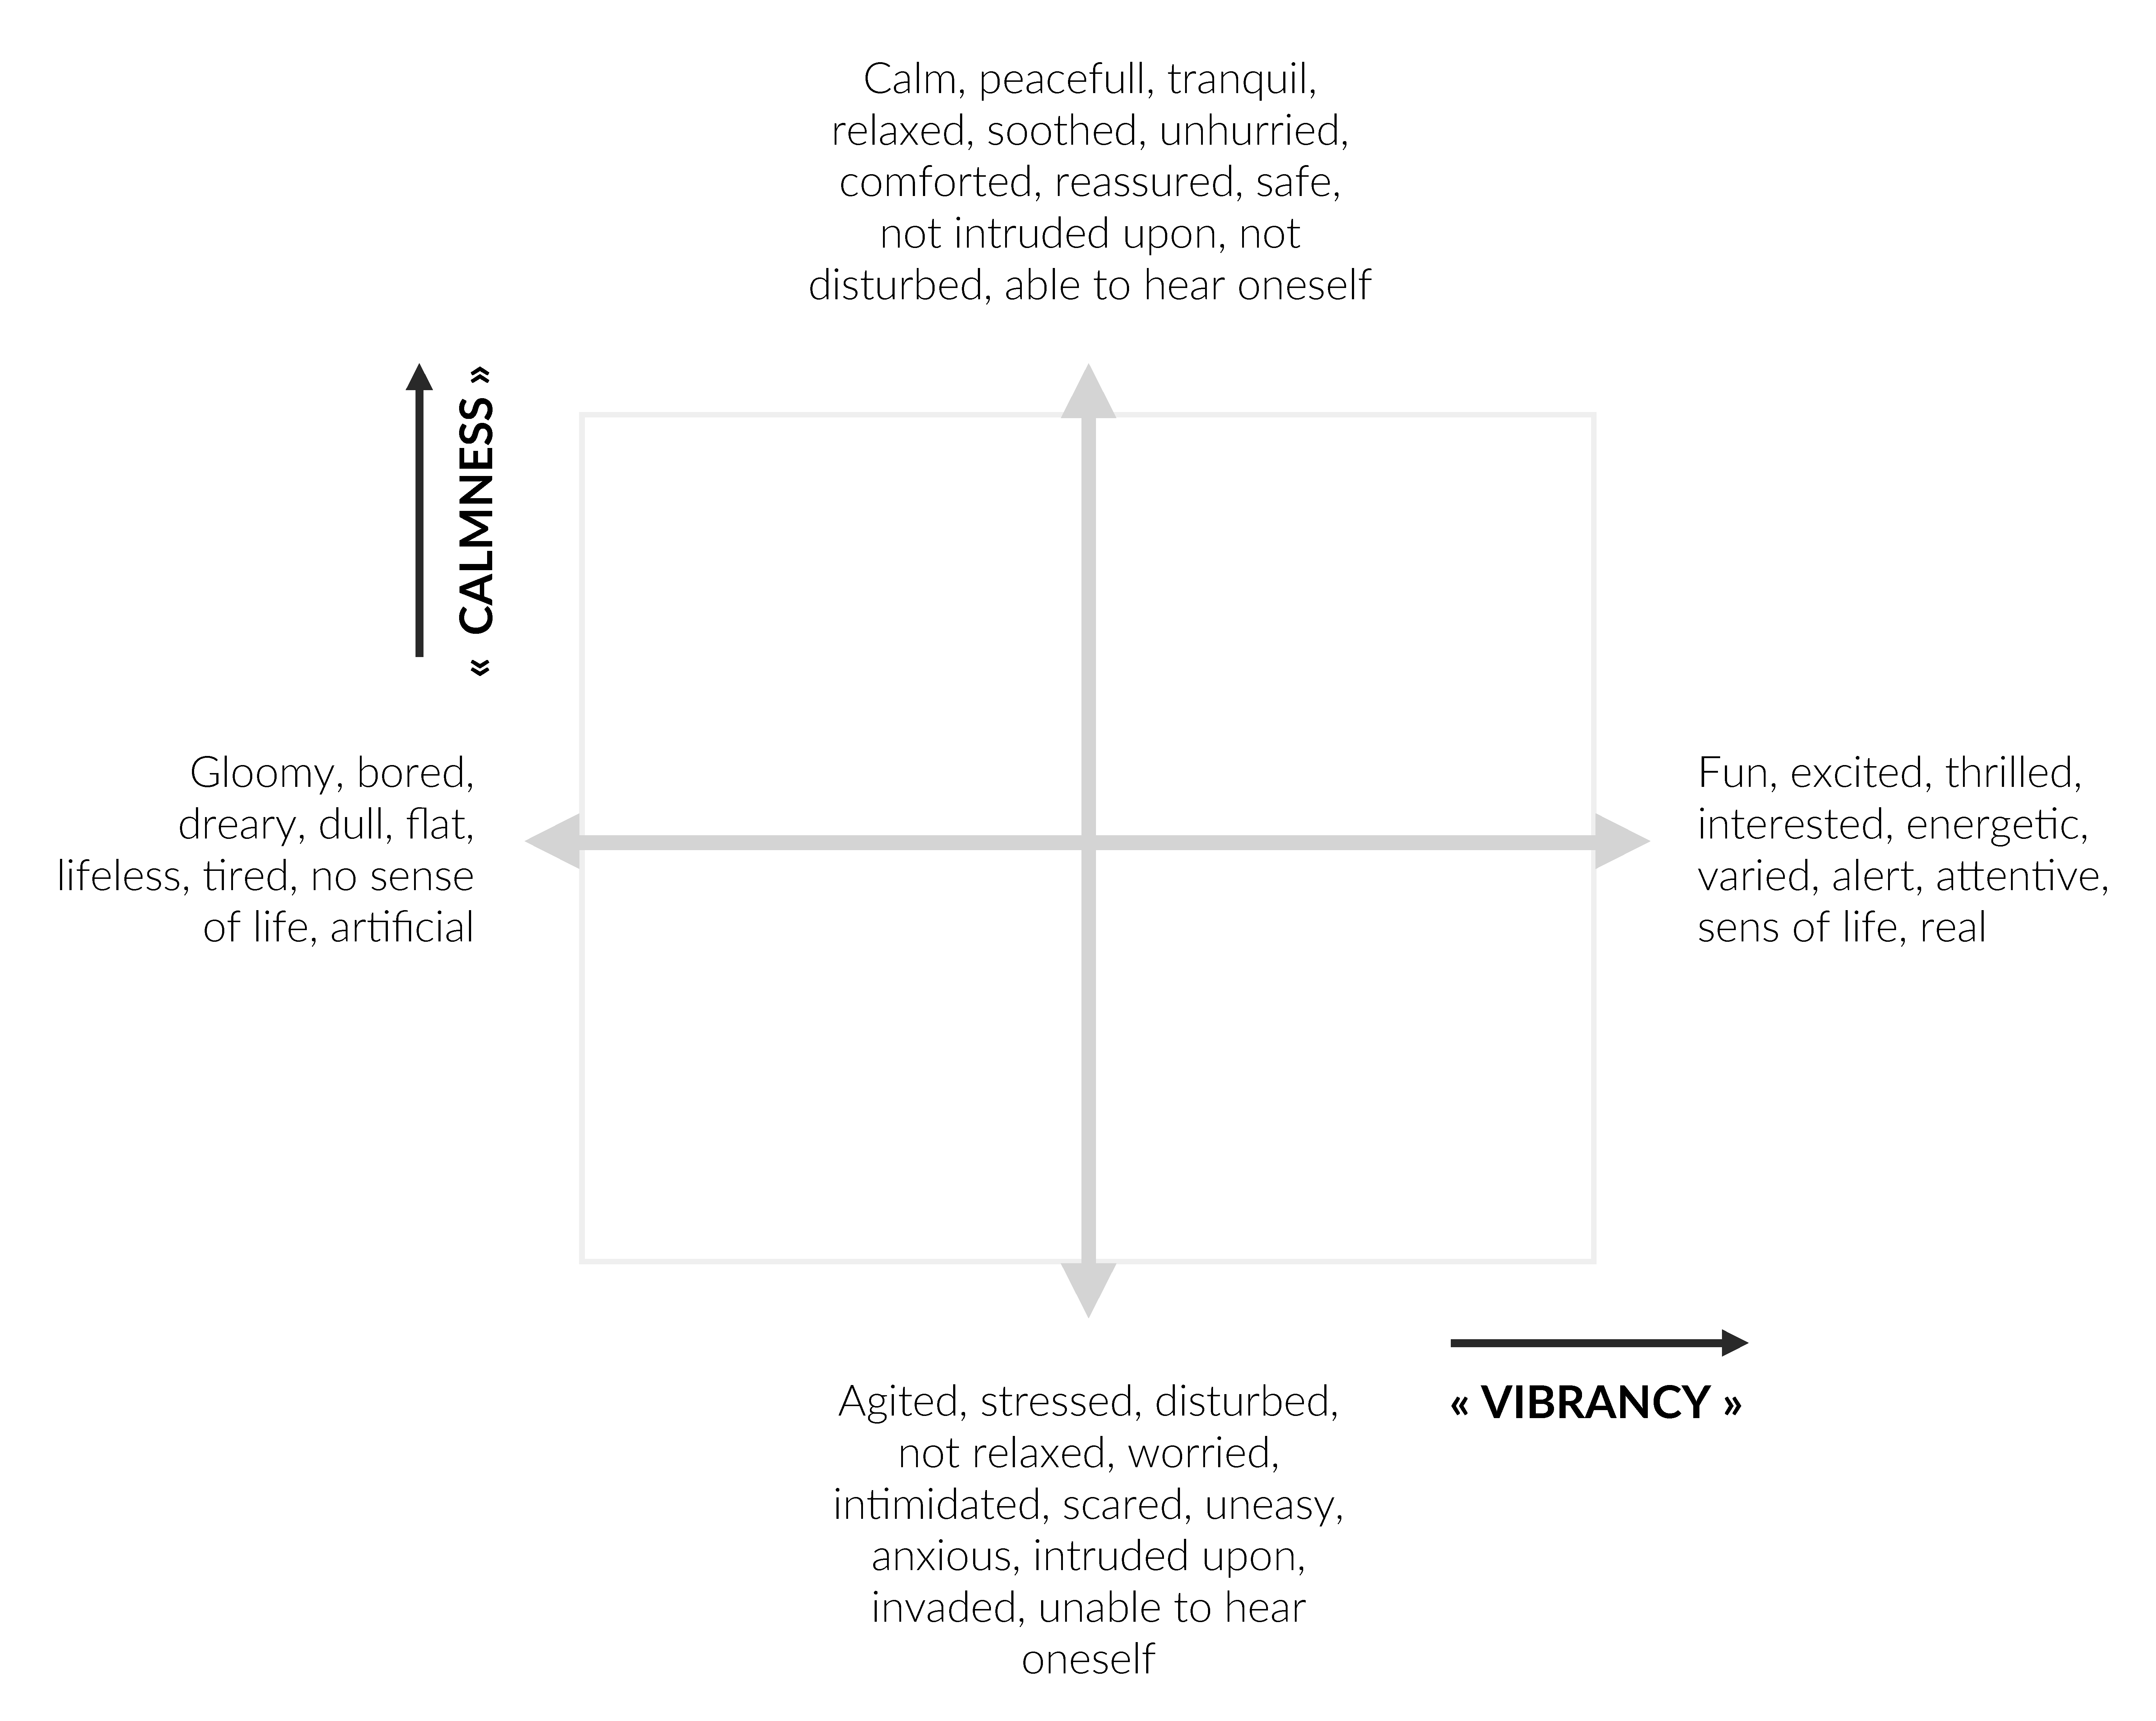
\includegraphics[width=.8\linewidth]{gfx/ch_3/calmVibran}
        \caption{Les dimensions de calme et de dynamisme permettant de caractériser l'environnement sonore urbain, d'après \citep{cain2013development}}\label{fig:calmVibran}
\end{figure}

\subsubsection{Autre descripteurs}

\gl{G0: \citep{kang2010semantic} autres} \\
\gl{G1: \citep{botteldooren2006temporal} music}

\subsubsection{Influence d'attributs extra-sonores}
\label{sec:ch3_contexteDimension}

Comme les exemples précédents le suggèrent, la perception d'un paysage sonore, et \emph{a fortiori} les processus cognitifs activés, sont très liés à un contexte.

Les recherches sur les paysages sonores ont permis de montrer que les qualités sonores d'un environnement dépendent, entre autre, d'un contexte environnemental (température, chaleur, humidité), \citep{meng2013field,jeon2011non}, relatif au sujet (age, sexe) ainsi qu'à sa sphère socio-culturelle
\citep{hall2013exploratory,yu2010factors,guillen2007importance}, relatif à la configuration spatiale du lieu d'exposition  \citep{hall2013exploratory}, au éléments visuels \citep{de2006quiet,guillen2007importance}, ainsi que d'un contexte de ``\,justesse\,'' (\emph{appropriateness}) \citep{nielbo2013investigating,de2006quiet}, \ie~la manière dont l'environnement sonore s'accorde avec l'activité du lieu.
 
\subsubsection{Réponse physiologique}

\gl{TODO:  \citep{hume2013physiological}}

\subsection{Catégoriser les sources et paysages sonores}
\label{sec:ch3_catSourceSoundScape}

\subsubsection{Catégories de sources sonores}
\label{sec:ch3_catSource}

Parmi les travaux les plus influents sur la catégorisation des sources sonores, on trouve ceux de W. W. Gaver \citep{gaver1993world,gaver1993we}. Se plaçant dans le cadre de l'``\,écoute de tout les jours\,'' (\cf~Section~\ref{sec:ch3_ecoute}), il propose d'envisager le problème sous un angle phénoménologique, en considérant l'action physique à l'origine, plutôt que l'objet. L'action étant très dépendante de la nature physique de l'objet, il trie les causes suivant trois types d'objets:

\begin{itemize}
\item solide : heurter, gratter, rouler, déformer;
\item liquide : goutter, éclabousser, clapoter;
\item gaz : exploser, souffler.
\end{itemize} 

D'autres études ont montré l'importance des phénomènes physiques originels dans les processus de catégorisation et d'interprétation des sons \citep{marcell2000confrontation,lemaitre2010listener}. \citep{houix_lexical_2012} notamment demande à des sujets de catégoriser librement 60 sons environnementaux en se concentrant sur l'action, et de commenter leurs groupes. Une analyse des groupements révèle que la catégorisation s'opère suivant deux étages hiérarchisés, le premier, le plus général, comprenant des catégories d'objets très proches à celles proposées par Gaver (Solide, Liquide, Gaz et Machine), et le deuxième, plus spécifique, comprenant des catégories d'actions. Une seconde expérience similaire, réalisée uniquement sur des objets solides, montre que la nature du pattern temporel (continu ou discret) résultant de l'action à l'origine du son influe de manière significative sur la catégorisation. Ce dernier point est également observé par \citep{gygi2007similarity}. Sur la base d'une matrice de similarité obtenue à partir de comparaisons par paires, et via un positionnement multidimensionnel en trois dimensions, Gygi~\al montre que les sons s'organisent en trois clusters incluant les sons harmoniques, les sons d'impacts (discret) et les sons continus. Une épreuve de catégorisation semi-libre  (les sujets devant réaliser au minimum 5 clusters), avec verbalisation pratiquée dans la même étude, montre par ailleurs que les sujets catégorisent les sons principalement en fonction du type de sources (animaux, homme, véhicule, mécanique, musique, eau), moins fréquemment en fonction du contexte et du lieu (extérieur, sport, bar) et rarement sur la base de caractéristiques physiques isolées (hauteur, fréquence) ou d'émotions ressenties (ennuyeux, alarmant)

L'influence de la nature de la source, et de sa sémantique associée, sur les processus de catégorisation a particulièrement été étudiée. A partir d'une étude de 35 papiers traitant de catégories sonores, \citep{niessen2010categories} établissent une liste de 20 catégories de sons les plus citées. La liste est présentée dans le Tableau~\ref{tab:categoNiessen}.

\begin{table}[t]
\centering
\begin{tabular}{ccc}    
\multicolumn{3}{l}{Nom des catégories les plus citées} \\             
\hline
Sons naturels                    & Voix       & Voiture\\
Sons humains                     & Enfant     & Machine\\
Sons technologiques/artificielles & Cloche     & Vent \\
Trafic                           & Background & Aboiement chien\\
Oiseaux                          & Événement  & Bruits de pas\\
Musique                          & Avion      & \\
Travaux                          & Eaux       & \\
\hline
\end{tabular}
\vspace{0.5mm}
\caption{Les catégories sonores les plus citées, d'après \citep{niessen2010categories}}
\label{tab:categoNiessen}
\end{table}

La grande majorité de ces catégories sont des catégories de sources sonores. Seules deux font référence à des catégories d'objets sonores abstraits (Événement, \emph{Background}). Ces catégories de sources ne s'expriment pas toutes au même niveau d'abstraction. Certaines sont précises (\emph{Aboiement chien}), d'autres sont très larges (\emph{Sons naturels}). Par ailleurs, certaines sont incluses dans d'autres (\emph{Bruits de pas}<\emph{Sons humain}), les trois catégories ayant le périmètre le plus large, et englobant toutes les autres sont  \emph{Sons naturels}, \emph{Sons humains} et \emph{Sons technologiques/artificiels}. Comme nous allons le voir (\cf~Section~\ref{sec:ch3_catsoundscape} et~\ref{sec:ch3_contribSource}) c'est en partie suivant ce découpage catégoriel que s'opère la perception de l'environnement.

Plusieurs études se basent sur une analyse linguistique de descriptions spontanées et libres d'environnements sonores, afin d'établir des catégories de sources sonores. Dans ces études, il est d'usage de demander explicitement au sujet de distinguer les aspects plaisants et désagréables du paysage étudié.

En réalisant une étude \emph{in situ} d'environnements de parcs, \citep{szeremeta2009analysis} mettent en évidence 9 catégories de sources sonores. Certaines sont systématiquement positivement connotées (\emph{oiseaux}, \emph{nature}), d'autres négativement connotées (\emph{machine}, \emph{alarme/signaux}, \emph{train}), d'autres encore peuvent être jugées soit positives soit négatives comme \emph{personne} (majoritairement positive), \emph{trafic véhicule} (majoritairement négative), \emph{musique}, \emph{trafic aérien}.

L'étude de \citep{guastavino2006ideal} utilise une méthode d'analyse similaire, mais en demandant aux sujets de décrire un environnement urbain idéal (plaisant), sur la base de leur mémoire uniquement. Des résultats similaires sont observés, \ie~les catégories \emph{oiseaux} et \emph{nature} sont systématiquement positivement perçues, les catégories \emph{klaxon} et \emph{travaux} négativement perçues, les catégories \emph{personne} (majoritairement positivement connotée) et \emph{musique} ayant une connotation variable.

L'auteur fait remarquer que les sujets décrivent les sons en s'appuyant sur la source émettrice de ces derniers. Il y a donc une assimilation entre l'objet et le phénomène acoustique. En conséquence la sémantique (le sens) liée à l'objet intervient dans le processus perceptif (dans ce cas le jugement hédonique) au même titre que les propriétés acoustiques. L'observation des appréciations inhérentes aux catégories de véhicules vont dans ce sens: les catégories \emph{trafic} (\emph{voiture}, \emph{moto/scooter}, \emph{camion}) sont systématiquement négativement perçues, à la différence des catégories \emph{transports publics} (\emph{bus} et \emph{train}), toujours bien perçues. La représentation positive que nous avons des \emph{bus} fait que ces sons, bien que proches de ceux de véhicules individuels, sont largement bien acceptés.  

Nous noterons cependant que l'étude de \citep{guastavino2006ideal} est réalisée sans support sonore, les sujets n'ayant que leur mémoire pour se représenter l'environnement urbain idéal. On peut penser que dans ce cas, les attributs sémantiques sont particulièrement sollicités. Nous approfondissons ce point à la section~\ref{sec:ch5_anaQualiSem}.  

\subsubsection{Catégories de paysages sonores}
\label{sec:ch3_catsoundscape}

Outre les catégories de sources sonores, plusieurs études s’intéressent à la formation de catégories d'objets plus complexes, les paysages sonores.

V. Maffiolo \citep{maffiolo_caracterisation_1999} montre l'existence de deux processus distincts engagés, en fonction de la capacité de l'auditeur à identifier des événements sonores. Dans cette étude, les sujets doivent 1) catégoriser des enregistrements d'environnements sonores urbains, et 2) décrire les groupements effectués. A partir d'une analyse linguistique des descriptions verbales, Maffiolo montre l'existence de deux catégories cognitives abstraites d'environnements sonores respectivement appelées: ``\,les séquences événementielles\,'' et ``\,les séquences amorphes\,''. Les séquences événementielles sont des environnements composés d'événements saillants et identifiables (\emph{démarrage de voiture}, \emph{voix d'homme}). Les séquences amorphes sont des environnements dont il est difficile d'isoler des éléments distincts.

Chacune de ces catégories a été sous catégorisée suivant différentes stratégies:

\begin{itemize}
\item les scènes événementielles ont été sous-catégorisées en fonction:
\begin{enumerate}
\item du type de source présent;
\item de la qualité affective de l'environnement (agréable, désagréable, ennuyant, agressif, insupportable, calme).
\end{enumerate}
\item les scènes amorphes ont été sous-catégorisées en fonction:
\begin{enumerate}
\item de l'agrément perçu (agréable/désagréable);
\item de l'évaluation des propriétés acoustiques à savoir l'intensité sonore, le contenu spectral (haute basse fréquence) et la structure temporelle (continu, discontinu).
\end{enumerate}
\end{itemize}

On remarque ainsi que les scènes événementielles profitent d'une analyse descriptive basée sur l'identification des sources sonores, alors que les scènes amorphes bénéficient d'une analyse holistique, à partir d'indicateurs acoustiques (subjectifs) globaux. On note que les deux catégories suscitent un jugement hédonique (plaisant/non-plaisant).

Cette distinction (événementiel/amorphe) s'opère aussi au niveau de la source sonore. Analysant des descriptions libres des sources sonores peuplant l’environnement urbains, Guastavino montre que les descriptions des sons à basse fréquence peuvent se diviser en deux catégories appelées ``\,événements sonores\,'' et ``\,bruit de fonds\,''. Dans les derniers, aucune source ne peut être identifiée.

Raimbault et Dubois \citep{raimbault2005urban}, combinant les résultats obtenus par trois thèses \citep{maffiolo_caracterisation_1999, raimbault2002simulation, guastavino_etude_2003}, montrent que la catégorisation des paysages sonores s'opère, suivant leurs compositions, en termes de sources sonores (\cf~Figure~\ref{fig:catSoundscapeRaimbault}). Une première distinction s'opère entre d'un coté les paysages sonores comportant des sons de \emph{transports motorisés} et/ou de \emph{travaux}, et  de l'autre, des paysages sonores comportant des sons suggérant une présence humaine. Ces derniers se subdivisent encore entre d'une part les paysages ``\,vivant\,'', et d'autre part les paysages ``\,relaxant\,'' composés également de sons de \emph{nature}. Le rôle prédominant joué par l'activité humaine dans la catégorisation des environnements était déjà pressentie par  Schaefer \citep{schafer1977tuning}.

Des résultats très similaires sont obtenus par \citep{guastavino2007categorization}. Passant par une tâche de catégorisation libre avec verbalisation, Guastavino montre que la catégorisation s'opère suivant la présence/absence de sons d'origine humaine, ainsi que sur un jugement hédonique des sources. La présence de sons humains agit sur deux niveaux, 1) les environnements sont divisés entre ceux dominés par les sons humains, et ceux dominés par les sons mécaniques. 2) Les premiers se subdivisent en fonction de l'activité et du lieu (parc calme, marché actif). Les seconds se subdivisent encore à partir de la présence ou non de sons humains.

\begin{figure}[t]
        \myfloatalign
        \includegraphics[width=\linewidth]{gfx/ch_3/categoRaimbault}
        \caption{Catégorisation des paysages sonores urbains, d'après \citep{raimbault2005urban}}\label{fig:catSoundscapeRaimbault}
\end{figure}

\subsection{Classifier les sources et environnements sonores}

Contrairement à la section précédente, où il est question de catégories, \ie~représentation mentale, nous traitons ici de classes. Par classe on entend un groupe d'objets qui ne fait pas référence à une entité mentale particulière, mais dont le regroupement vient d'une volonté de classer/d'organiser des environnements, ou des sources, suivant leurs caractéristiques physiques, morphologiques, ou encore suivant leurs fonctions. Le but est alors, sur la base de descripteurs objectifs, d'étudier les similarités existant entre ces groupes, (\cf~Section~\ref{sec:appDimensionelle}).


\subsubsection{Classes de sources sonores}

Un des buts premiers des études sur les classes sonores est d'établir la typologie complète de tous les types de sources peuplant un environnement donné.

Sur la base de l'étude de \citep{raimbault2005urban}, et dans l'idée de proposer une nomenclature générique pour décrire les sources sonores présentes en milieu urbain, \citep{brown2011towards} propose une taxonomie reprise à la figure~\ref{fig:catSoundscapeBrown}. Cette classification est centrée sur l'objet. En partant de la taxonomie proposée par \citep{brown2011towards}, \citep{Salamon14} propose une nouvelle taxonomie, plus détaillée, centrée, elle, à la fois sur l'objet et sur l'action (\cf~Figure~\ref{fig:catSoundscapeSalamon}). Les auteurs partent de l'idée que la réalité sonore d'un objet diffère en fonction de son utilisation (\emph{passage de voiture}~\vs~\emph{freinage de voiture}~\vs~\emph{klaxon de voiture}). Pour rendre compte de ce fait,  certaines classes d'objets du plus bas niveau sont subdivisées en classes d'actions, labellisées par des verbes.

Outre organiser les sources, il est aussi utile de comprendre quelles sont les différences acoustiques qui peuvent se manifester entre plusieurs classes de sons. \citep{yang2013psychoacoustical}, sur la base d'indicateurs acoustiques et psychoacoustiques, compare des classes de sons provenant d'environnements urbains (\emph{musique}, \emph{mécaniques} et \emph{trafic}) et d'environnements naturels (\emph{eau}, \emph{vent} et \emph{oiseaux}). Chaque indicateur est calculé sur le signal, à l'aide d'une fenêtre glissante, et moyenné. En réalisant une analyse en composante principale sur ces indicateurs, les auteurs montrent que l'intensité (\emph{loudness  de Zwicker}), le contenu spectral \emph{sharpness} et la structure temporelle \emph{fluctuation} sont les trois principaux indicateurs permettant d'expliquer la variance entre ces différents types de sons. Ce fait avait déjà été observé dans d'autres études mêlant différents stimuli \citep{de2006quiet,botteldooren2006temporal}.


\begin{figure}[t]
        \myfloatalign
        \includegraphics[width=\linewidth]{gfx/ch_3/categoBrown}
        \caption{Taxonomie des sources sonores urbaines, d'après \citep{brown2011towards}}\label{fig:catSoundscapeBrown}
\end{figure}

\subsubsection{Classes de paysages sonores}
\label{sec:ch3_classePaysage}

Beaucoup d'études analysent l'existence de similarités entre environnements sonores à partir d'indicateurs quantitatifs, qu'ils soient objectifs \citep{rychtarikova2013soundscape}, subjectifs \citep{jeon2013soundwalk}, ou les deux à la fois \citep{torija2013application,ricciardi2015sound}. La méthodologie est presque toujours la même:

\begin{enumerate}
\item Pour chaque environnement, calculer des indicateurs acoustiques/psychoacoustiques, ou évaluer des indicateurs perceptifs à l'aide d'échelles sémantiques
\item Utiliser des outils de clustering afin d'établir des classes d'environnements similaires.
\end{enumerate}

Sur la base de descripteurs subjectifs uniquement, \citep{jeon2013soundwalk} identifient quatre classes comprenant respectivement, des environnements dominés par le bruit urbain, des environnements comprenant majoritairement des composantes naturelles, des environnements urbains ouverts (place), ou encore des environnements équilibrés (sons urbains et naturels). La distinction se fait en grande partie à partir d'indicateurs de préférence liés au confort acoustique, mais également à l'impression visuelle et à la configuration spatiale du lieu.  

Sur la base de descripteurs subjectifs et objectifs, \citep{torija2013application} établit 15 classes de paysages sonores. Il apparaît que la distinction correspond à des différences au niveau des sources sonores présentes/absentes (trafic, oiseaux, fontaine, moto, sirène, parc, humain). Parmi les indicateurs acoustiques, ceux tenant compte de la dynamique du niveau sonore (\emph{crest factor}) ainsi que du niveau des basses fréquences ($L$ à 125Hz) permettent à eux seuls d'expliquer 84\% de la variance des données. Les auteurs concluent que l'utilisation de descripteurs acoustiques peut permettre, seule, d'isoler les paysages sonores similaires, conclusion reprise par \citep{rychtarikova2013soundscape}.

\gl{TODO: contredire cette vérité}

\subsection{Contributions des différentes sources sonores}
\label{sec:ch3_contribSource}

Comme nous l'avons vu, plusieurs études adoptant l'approche catégorielle ont permis de montrer que l'identification de certaines sources sonores, ainsi que leur sémantique associée, joue un rôle important dans l'évaluation perceptive des paysages, particulièrement au niveau de l'agrément perçu \citep{guastavino2006ideal,szeremeta2009analysis}.

\gl{TODO: l'écoute \citep{gaver1993world}}\\

Continuant dans ce sens, les études adoptant l'approche dimensionnelle cherchent de plus en plus à compléter les indicateurs globaux avec des indicateurs caractérisant les contributions spécifiques de différentes sources sonores. Pour ce faire, elles partent toutes d'une liste de catégories de sources pré-établie. A partir de cette liste, elles calculent des indicateurs acoustiques spécifiques à ces sources, et/ou demandent à des sujets d'en évaluer les caractéristiques perceptives.

En menant différentes études \emph{in situ} sur la qualité de différents environnements, \citep{nilsson2007acoustic,nilsson2007soundscape} montrent que l'identification des sources sonores permet de mieux prévoir la qualité globale de l'environnement que le niveau sonore. En particulier les sons \emph{technologique/mécanique} ont un impact négatif sur l'environnement alors que les sons \emph{naturels} ont un impact positif. Les sons \emph{humains} restent cependant neutre. De plus, l'étude montre que dans le cas d'une exposition modérée au bruit de trafic, l'ajout de sons positivement perçus (\emph{naturels} dans leur cas) peut potentiellement améliorer la qualité de l'environnement, une observation déjà effectuée par d'autres études \citep{hong2013designing,galbrun2012perceptual}. Cependant, pour une exposition élevée au bruit, une politique de réduction des niveaux est obligatoire.

\citep{defreville2004aactivity,lavandier2006contribution} évaluent l'impact séparé de différentes sources de trafic (\emph{voiture}, \emph{moto}, \emph{scooter}, \emph{bus}), de sons humains (\emph{voix adultes}, \emph{voix enfants}) et de sons naturels (\emph{oiseaux}) sur l'agrément perçu. Pour chacune de ces sources ils  calculent des indicateurs objectifs de niveaux ($L_{Aeq}$, $L_{A10}$) et de présence (nombre d’occurrences, pourcentage de temps présent), ainsi que des indicateurs perceptifs (présence, proéminence, proximité). Des indicateurs globaux relatifs au niveau (objectif: \emph{loudness de Zwicker}; subjectif: niveau perçu) sont également pris en comptes. La régression linéaire multiple est utilisée afin de mesurer l'influence des indicateurs sur l'agrément.

Que l'on considère les indicateurs subjectifs ou objectifs, l'utilisation combinée de l'indicateur de niveau global avec les indicateurs spécifiques aux différentes sources permet d'augmenter la capacité de prédiction de la qualité sonore, comparé à l'utilisation de l'indicateur de niveau global seul. Là encore les auteurs montrent que dans le cas où les environnements sont peu exposés au trafic, les sons d'\emph{oiseaux} et d'\emph{humain} ont un effet positif, la qualité augmentant en fonction de leur présence. Ils notent également que l'appréciation des \emph{voitures} diffère en fonction du type d'environnement: dans un parc, elles ont un effet négatif alors que dans une rue, elles sont comprises comme faisant partie de l'environnement et n'influencent pas (de manière individuelle) la qualité perçue.

Dans une étude d'envergure, comprenant 3400 réponses collectées sur deux villes (Paris et Milan), et utilisant une méthodologie proche de celle de \citep{lavandier2006contribution}, Ricciardi~\al \citep{ricciardi2015sound} testent plusieurs modèles permettant de prédire la qualité sonore. Ces modèles sont tous bâtis à partir d'indicateurs perceptifs globaux, sonores et visuels, ainsi que d'indicateurs perceptifs sonores spécifiques à différentes sources. Les modèles tenant compte des indicateurs visuels produisent des sorties corrélées à 72\% avec la qualité mesurée. Cette corrélation décroît à 58\% si l'on supprime les indicateurs visuels, et tombe à 19\% si l'on ne considère plus que le niveau sonore global (sans les indicateurs spécifiques aux sources). Les auteurs clusterisent les différents environnements sur la base de ces indicateurs. 6 classes sont mises à jours, les regroupements étant encore une fois relatifs à la présence/absence de diverses sources sonores. Plus spécifiquement, certains groupements sont liés:

\begin{enumerate}
\item à la possibilité de distinguer, ou non, des sources sonores dans les scènes (scènes événementielles~\vs~amorphes);
\item  à la présence majoritaire d'une classe de sons en particulier (\emph{trafic}, \emph{humain}, \emph{nature});
\item à la présence simultanée de plusieurs sources.
\end{enumerate}

En recalculant des modèles pour chacune des classes, les auteurs montrent que les indicateurs relatifs à des sources sont plus représentés dans le cas des modèles par classes, mais varient significativement d'une classe à l'autre. Par exemple, l’indicateur relatif aux sources d'\emph{oiseaux} n'apparaît, dans le modèle, que pour la classe dominée par des sons \emph{naturels}. Ces résultats questionnent l'utilité et l'efficacité d'une modélisation de la qualité sonore qui se voudrait générale, \ie~applicable pour tout type de situations et d'environnements.


\section{Événements et textures sonores}
\label{sec:ch3_eventTexture}

\subsection{Définition}
\label{sec:ch3_textureDef}

S'éloignant de l'approche des paysages sonores, plusieurs études se sont concentrées sur l'analyse perceptive d'un certain type de sons, appelés texture sonore.

Pour définir la texture sonore, nous nous appuyons sur la définition donnée par \citep[p. 25]{saint1995classification}:  

\begin{itemize}
\item ``\,les textures sonores sont des objet composites, formés d'éléments de base appelés atomes;\,''
\item ``\,les atomes apparaissent suivant un pattern haut-niveau pouvant être soit périodique (galop), soit aléatoire (pluie), voire les deux;\,''
\item ``\,les caractéristiques haut niveaux des textures restent constantes sur de longue périodes de temps, ce qui implique qu'elles ne peuvent comporter aucun message complexe;\,''
\item ``\,le pattern haut-niveau doit être présenté au moins une fois dans sa totalité pendant une période de temps n’excédant pas les quelques secondes. Cette période est nommée période d'attention (\emph{attention span}).\,''
\end{itemize}

Cette définition est avant tout morphologique, la texture étant définie en fonction de ses caractéristiques physiques. Cela vient, entre autre, du fait que la texture a d'abord été étudiée dans le cadre du traitement du signal, beaucoup d'applications multimédia ayant besoin de  modèles permettant de synthétiser de tels sons \citep{schwarz2011state}. La notion de texture s'oppose intuitivement à celle d'événement sonore et de séquence d'événements. Par opposition, l'événement est vu comme un élément discret, un son court et non homogène.

C'est par la notion d'information transmise que semble se faire la distinction entre texture et séquence d'événements. Les caractéristiques des textures restant stables au cours du temps, l'information transmise finit éventuellement par atteindre une asymptote. A contrario, une succession d'événements distincts, comme c'est le cas pour une séquence musicale ou de parole, transmet de plus en plus d'informations dans le temps (\cf~Figure~\ref{fig:texture}). En poussant le raisonnement à l’extrême, le bruit blanc peut être vu comme la représentation la plus ``\,pure\,'' d'une texture, ce dernier étant porteur d'une information très limitée.

Cette dimension événement/texture est orthogonale à celle de ``\,bruit de fond\,'' / ``\,événements de premier plan\,'' (\emph{background}/\emph{foreground}), utilisée dans le langage courant pour discriminer l’environnement urbain. Concernant les notions de background et de \emph{foreground}, nous considérons que l'une, et l'autre peuvent être vues comme des flux auditifs, ces derniers pouvant être composés à la fois de textures et d’événements regroupés dans le but de faciliter le traitement auditif de la scène.

\begin{figure}[t]
        \myfloatalign
        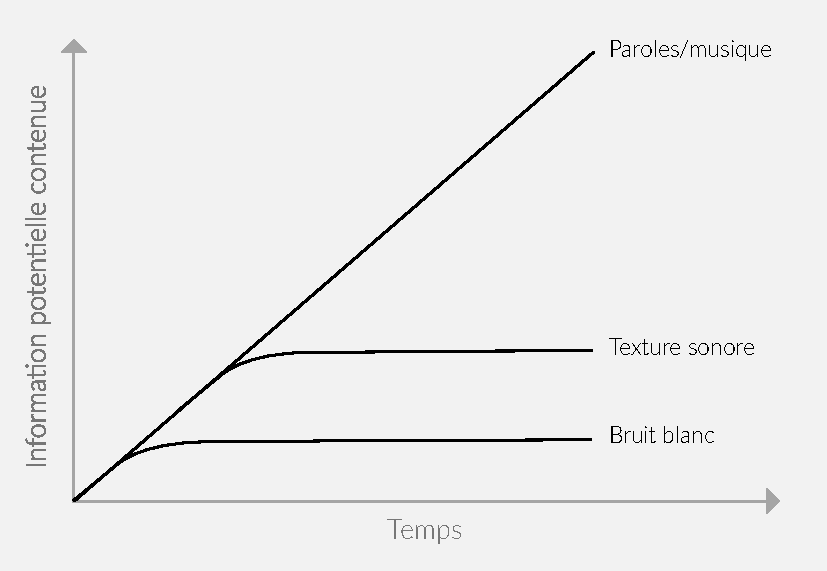
\includegraphics[width=.8\linewidth]{gfx/ch_3/texture}
        \caption[Information potentielle contenue dans les séquences d'événements, les textures, et le bruit]{Information potentielle contenue dans les séquences d'événements, les textures, et le bruit. D'après \citep{saint1995classification}}\label{fig:texture}
\end{figure}

\subsection{Percevoir les textures}
\label{sec:ch3_texturePerception}

Contrairement aux événements sonores, la texture est un objet simple, dont le traitement cognitif ne requiert pas une analyse poussée. 

Cela a été mis en évidence par Josh H. McDermott et ses-co auteurs \citep{mcdermott2011sound,mcdermott2013summary}. S'inspirant du fonctionnement de l'oreille humaine, et notamment des processus auditifs intervenant depuis la cochlée, jusqu'au thalamus, ils ont pu établir un modèle permettant de re-synthétiser des textures sonores en ne se servant que de statistiques simples, calculées à partir de représentations temps-fréquence de signaux de textures enregistrés. 

Dans une première expérience \citep{mcdermott2011sound}, la capacité des sujets à identifier les textures synthétisées a été testée. Les résultats ont montré que les sons de synthèse étaient aussi bien identifiés que les sons enregistrés. McDermott démontre ainsi qu'une information résumée sous la forme de statistiques, est utile, d'un point de vue cognitif, à la reconnaissance. Dans le cas des textures, ces statistiques constituent même l'unique information disponible, le système auditif ayant fait fi de toute autre représentation plus détaillée \citep{nelken2013ear}.

Dans une seconde expérience \citep{mcdermott2013summary}, les sujets ont dû reconnaître, parmi une triade de sons synthétisés, celui produit par une source différente (\ie~un type de texture différent, \cf~Figure~\ref{fig:textureMcder}). Les résultats ont montré que la capacité de discrimination est fonction de la durée des textures. Plus cette dernière est élevée, plus la capacité à discriminer est importante. Ce constat valide les hypothèses formulées par \citep{saint1995classification} sur l'existence d'une période d'attention, nécessaire au cerveau afin de percevoir le stimuli comme une texture. Ces résultats ont aussi montré que le processus de traitement de l'information sonore comprend une prise de décision quant à la nature des stimuli, décision qui va  ensuite influer sur la manière d'analyser l'information montante. L'expérience prouve que cette prise de décision n'a rien d'anodine, car, dans le cas où le cerveau perçoit une texture, il décide sciemment de dégrader l'information, en la résumant de manière statistique.

Le fait qu'un jugement perceptif s'améliore avec la durée des stimuli est un principe bien connu en perception des sons \citep{moore1973frequency}. Une troisième expérience de \citep{mcdermott2013summary} a montré cependant que cette vérité n'était pas toujours vérifiée. Au cours de cette expérience, les sujets, soumis à trois exemplaires d'un même type de texture (\eg~trois sons synthétisés de pluie), dont deux étaient produits à partir des mêmes statistiques extraites, ont du identifier le troisième, issu de statistiques différentes (Figure~\ref{fig:textureMcder}). Les résultats ont montré que la capacité des sujets à discriminer le bon stimulus décroît avec la durée des stimuli. Ce fait, qui peut sembler paradoxal, est une conséquence directe du choix du cerveau de ne traiter les textures que sur la base de statistiques. Partant du principe que le signal sonore est analysé suivant des fenêtres d'intégrations successives \citep{yabe1998temporal,poeppel2003analysis}, plus les stimuli sont longs, plus le système auditif est confiant dans le fait qu'il a à faire à des textures, et plus il tend à conserver une information réduite. La réduction de cette information finit éventuellement par gommer les différences fines qui existent entre les stimuli, ce qui ne permet plus de faire la distinction entre eux.


\begin{figure}[t]
        \myfloatalign
        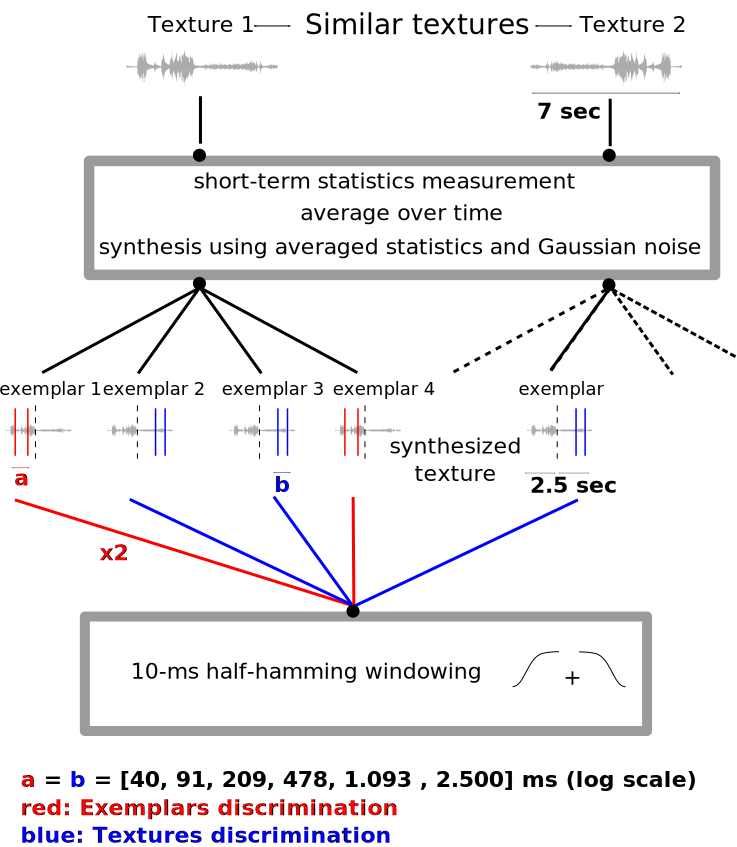
\includegraphics[width=.8\linewidth]{gfx/ch_3/mcder}
        \caption[Plannification expérimentale de l'expérience de discrimination de textures sonores et d'exemplaires de textures sonores]{Plannification expérientale des expériences de discrimination de textures sonores et d'exemplaires de textures sonores menées par \citep{mcdermott2013summary}}\label{fig:textureMcder}
\end{figure}

Une des avancés majeures de ces études est qu'elles apportent de nouvelles réponses sur la nature des représentations sonores stockées en mémoire. Dans le cas des textures, il s'agirait ainsi de descripteurs bas-niveaux, résumés sous la forme de statistiques simples. Cette découverte fait sens d'un point de vue écologique, car elle respecte le principe d'économie de moyens. Le cerveau, reconnaissant que les caractéristiques des textures n'évoluent pas au cours du temps, ne conserve en mémoire qu'une information condensée, qui lui permet pourtant de traiter des sons potentiellement longs. 

Il a été montré que le cerveau peut stocker bien plus que des statistiques. \citep{agus2010rapid} a mis en évidence qu'un bruit blanc, écouté de manière répétée, pouvait être reconnu encore plusieurs semaines après l'écoute, et ce parmi d'autres bruits blancs. Dans ce cas le cerveau emmagasine bien la totalité du signal acoustique.

\subsection{Discussions}
\label{sec:ch3_textureDiscussion}

\gl{TODO: terminer sur une discussion "texture, un groupe d'evt qui ont perdu leur signification individuelle" + "importance de l'attention span" (dire que ce point a été étudié: introduire l'expérience) + "problème avec le bruit blanc\citep{agus2010rapid}, texture non informatif mais pourtant stockée en totalité par le cerveau"}


\begin{figure}[t]
        \myfloatalign
        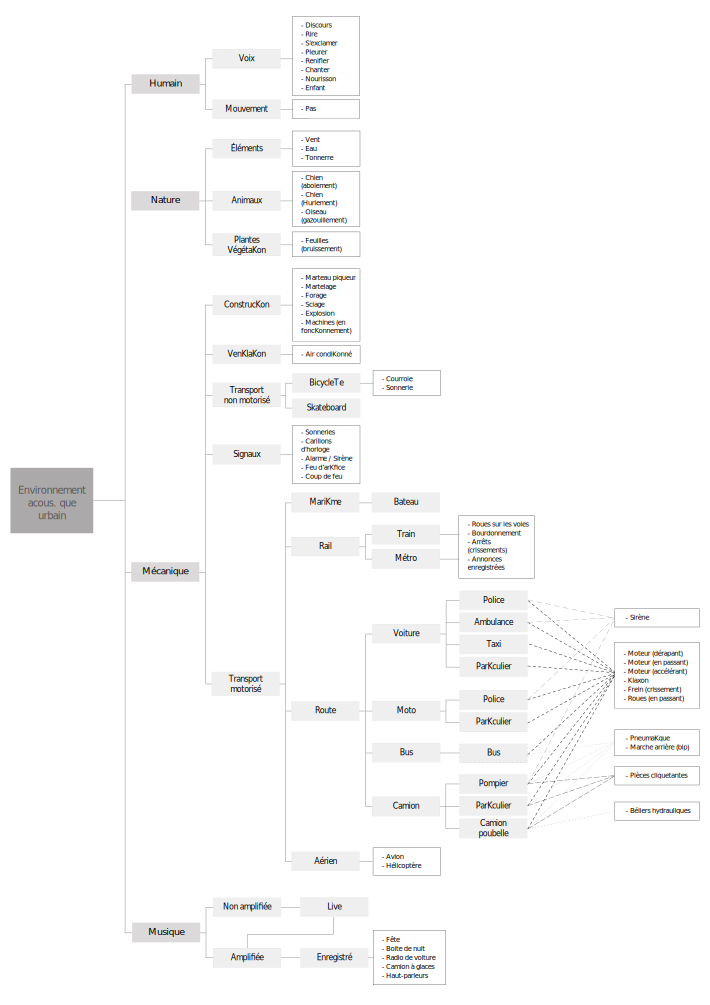
\includegraphics[width=\linewidth]{gfx/ch_3/categoSalamon}
        \caption{Taxonomie des sources sonores urbaines, d'après \citep{Salamon14}}\label{fig:catSoundscapeSalamon}
\end{figure}



%*****************************************
%*****************************************
%*****************************************
%*****************************************
%*****************************************
